\documentclass[a4paper,10pt]{article}
\setcounter{page}{1}

\tolerance=2000  % Allow slightly worse spacing
\pretolerance=1000  % Reduce aggressive line breaking

%%% The following commands load some necessary LaTeX packages
\usepackage{graphicx}
\usepackage{amsmath}
\usepackage{amssymb}
\usepackage{hyperref}
\usepackage{enumitem}
\usepackage{mathtools}
\usepackage{xfrac}

\usepackage{siunitx} % For units
\sisetup{per-mode=fraction}  % Forces fraction format

\usepackage{natbib}  % Use natbib for better citation styles

% For two-column layout
\usepackage{multicol} 
\usepackage{float}

%%%% These are for section titles:
\usepackage{titlesec}

\titleformat{\section}{\normalfont\Large\bfseries\MakeUppercase}{\thesection}{1em}{}
\titleformat{\subsection}{\normalfont\large\bfseries\MakeUppercase}{\thesubsection}{1em}{}
\titleformat{\subsubsection}{\normalfont\normalsize\bfseries\MakeUppercase}{\thesubsubsection}{1em}{}

%%% The following command sets margin sizes
\usepackage[top=1in, bottom=1in, left=0.75in, right=0.75in]{geometry}

%%% The following two commands set the font to Helvetica, which is close to Arial
\renewcommand{\familydefault}{\sfdefault}
\usepackage{helvet}

%%%% The following commands control the header of each page
\usepackage{fancyhdr}
\pagestyle{fancy}
\fancyhf{}
\fancyhead[L]{Proceedings of the URECA@NTU 2024-25}
\fancyfoot[C]{\thepage}
%%%%%%%%%%%%%%%%%%%%%%%%%%%%%%%%


% \usepackage{etoolbox}
% \renewcommand{\abstractname}{\textbf{\textit{Abstract}}}

%%%% The following commands control the abstract's format
\makeatletter
\renewenvironment{abstract}{
    \small
\noindent\textbf{\textit{\abstractname}}.\hspace{1em}} % Bold and italic "Abstract" followed by a dot and space
{}
\makeatother
%%%%%%%%%%%%%%%%%%%%%%%%%%%%%%%%%%%%%%%%%%%%


\usepackage[parfill]{parskip} % Removes paragraph indent and adds spacing between paragraphs
\usepackage{setspace}

\setlength{\parskip}{0.5\baselineskip} % Set spacing between paragraphs to 0.5 times the line height
\setlength{\parindent}{0pt} % Set paragraph indent to 0



%%%%% The following commands control the title of the paper and the authors' names
\title{Swarming Behavior in Honeybees}
\date{}
\author{
    {Lim Jia Qing} \\
    College of Computing and Data Science  \\
    \and
    {Asst Prof Yong Ee Hou} \\
    School of Physical and Mathematical Sciences \\
}

%%%%%%%%%%%%%%%%%%%%%%%%%%%%%%%%%%%%%%%%%

\begin{document}


%%%% Uncomment and insert the date if needed
% \date{}
\maketitle

\begin{multicols}{2}

    \begin{abstract}
        Self-assembly pervades nature, from the coalescence of iron oxide nanoparticles
        to the collective motion of flocks of birds. To understand self-assembly, we
        devised a set of simple local rules to simulate the swarming of Western
        honey bees (\textit{Apis mellifera}), thereby giving rise to a spectrum of
        interesting emergent states characterised by their morphology and behavior.
        Parameterised by two variables, a \textit{crawl rate} (how fast bees attached
        to the wooden board advance towards the queen) and a \textit{climb rate} (how
        vigorously bees at the peripheral of the structure attempt to scale the inverted
        mount), we were able to yield structures akin to those recorded in the
        physical world. These findings were then corroborated with empirical data established
        in the literature. Our simulation reveals that at lower-density
        regions, a diagonally-centered square lattice is the prevalent structure, while
        at higher-density regions, this lattice breaks down into an amorphous mesh
        of bees with a higher degree of connectivity.
    \end{abstract}

% Include at least three keywords of phrases
    \textbf{Keywords:} self-assembly, simulation, physics

    \section{Introduction}

    In the material sciences, self-assembly has always been a popular tool to understand the
    coalescence of microscopic particles and molecules. With the rise in computational power in recent
    decades, the concept of self-assembly has also proven critical in designing \textit{artificial life}
    programs. Famous examples include cellular automaton \cite{fetecau2012mathematical} as well as
    the Boids program \cite{reynolds1987flocks}. Through a few simple principles implemented at
    the local level, we're able to give rise to astounding emergent group behavior that transcends
    the individual. In this paper, we'll be examining the swarming of Western honey bees
    (\textit{Apis mellifera}) through the lens of self-assembly.

    During reproduction, there are four distinct phases that honey bees go through \cite{grozinger2014molecules}.
    The first is the swarm exodus phase where they leave their current nest, followed by the migration
    phase where they initiate their search for a new site. When a suitable site is found, the
    bees form a temporary cluster. This inverted mount is known as a \textbf{bivouac}, and is
    the subject of study in this paper. Finally, when an alternative has been found, they
    enter the final phase (swarm liftoff) where they disassemble the structure and head towards
    the new location.

    \begin{figure}[H]
        \centering
        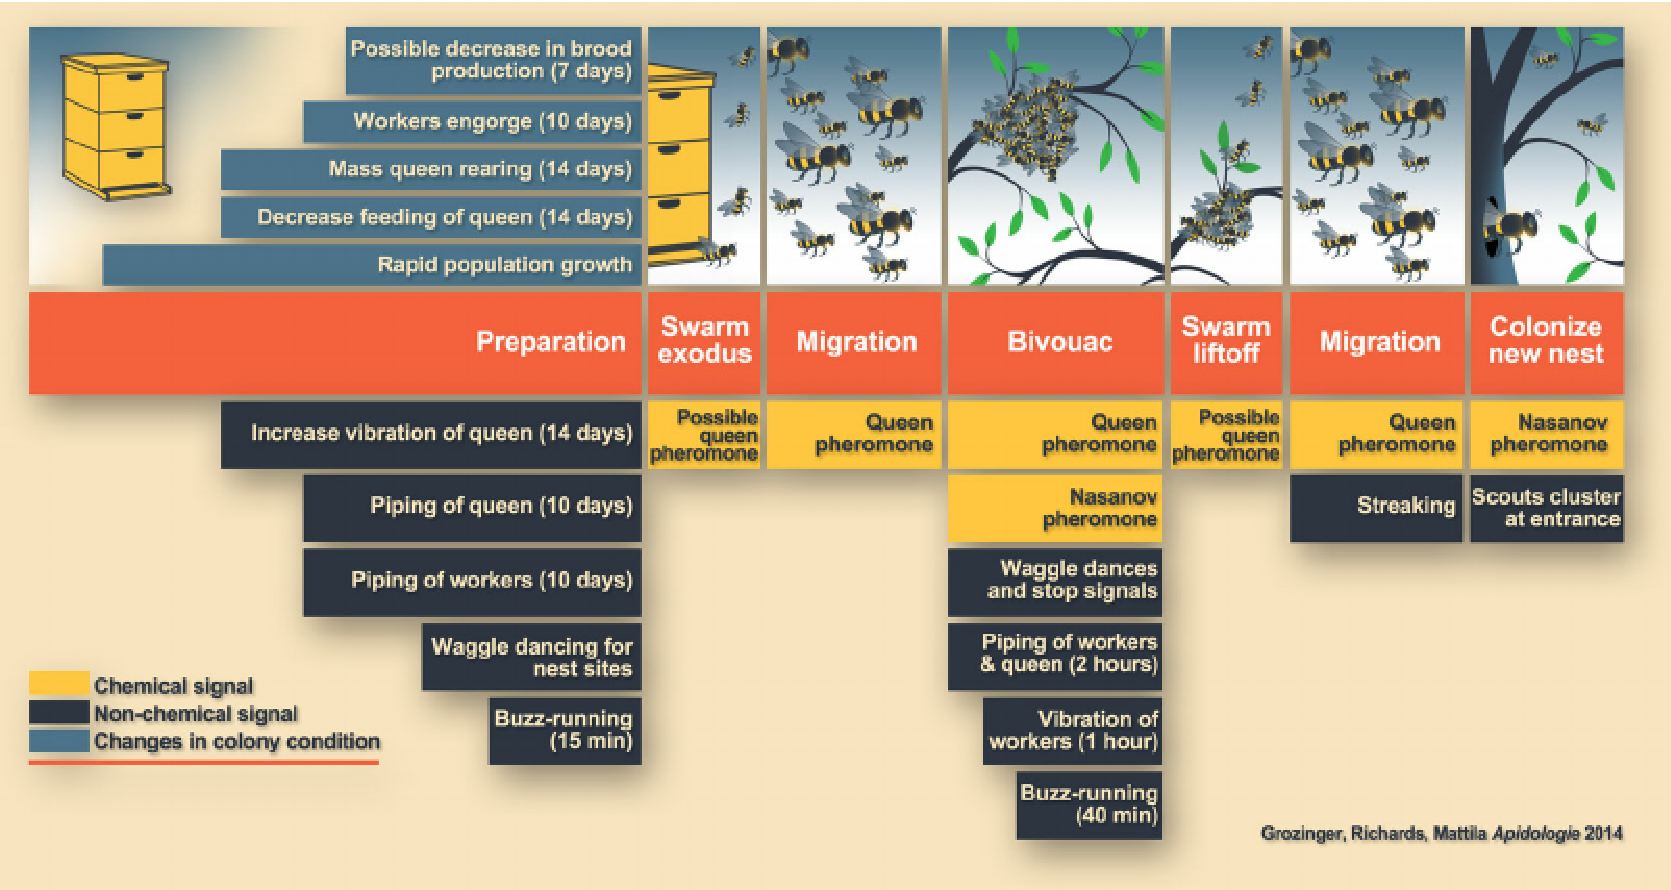
\includegraphics[width=\linewidth]{phases.pdf}
        \caption{An overview of the reproduction phases \cite{grozinger2014molecules}}
    \end{figure}


    \begin{figure}[H]
        \centering
        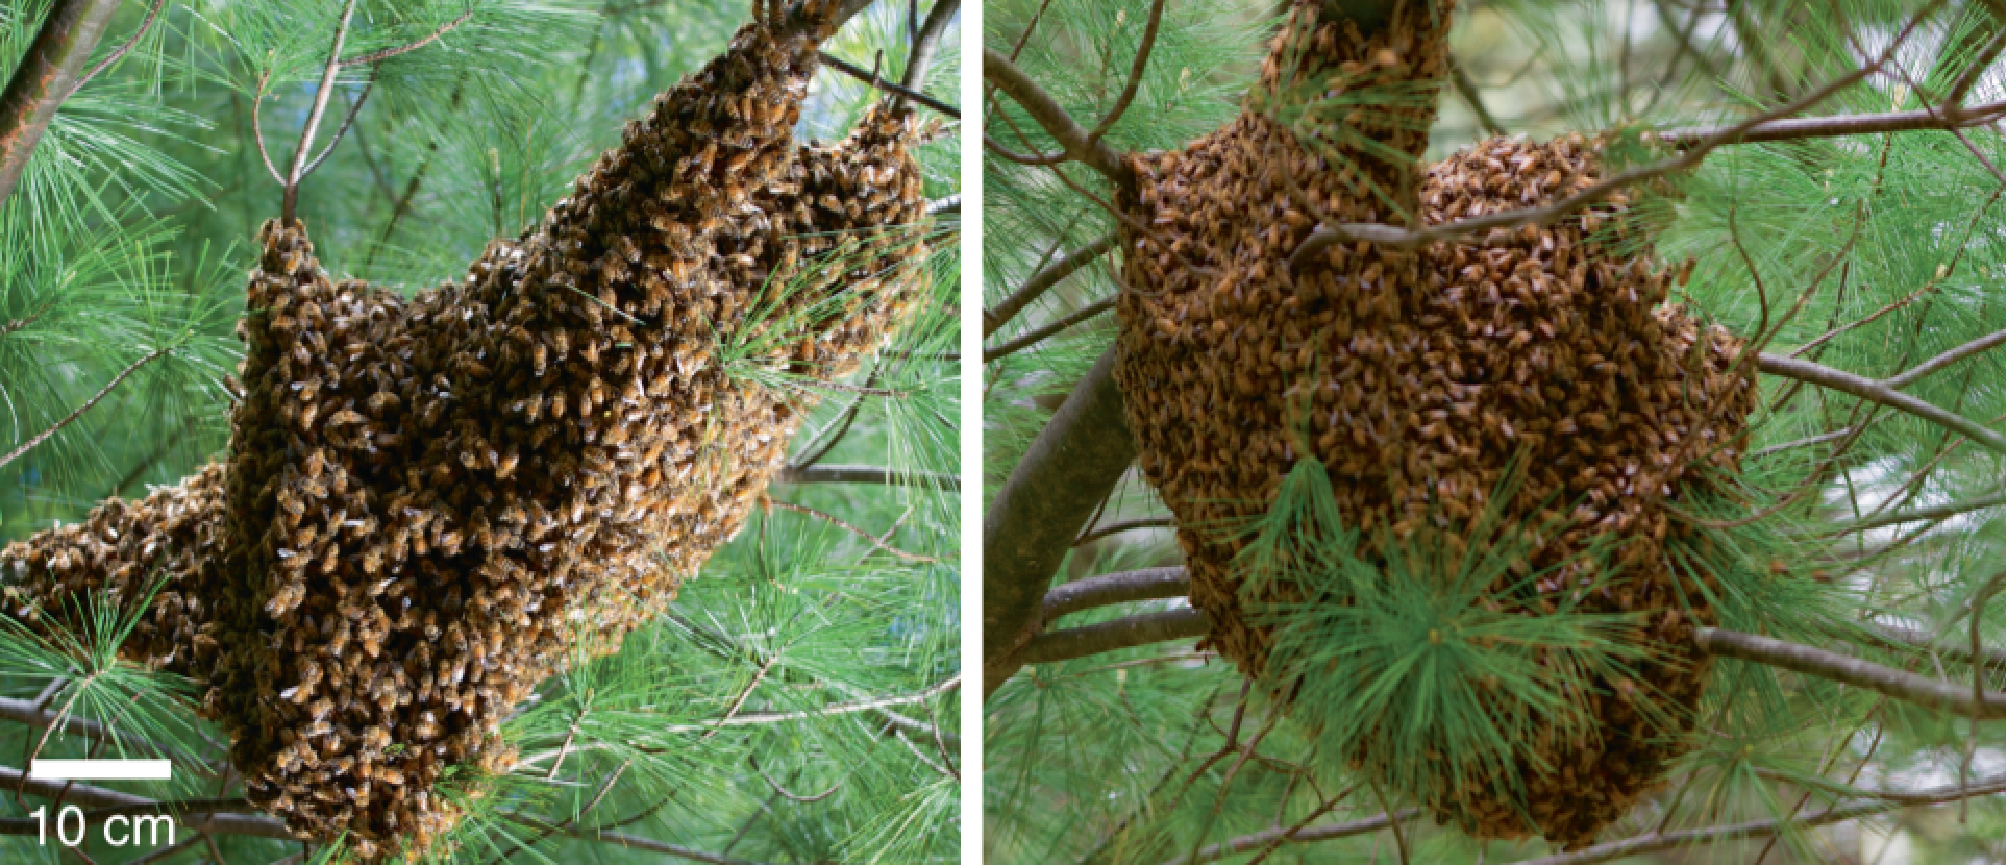
\includegraphics[width=\linewidth]{bivouac_exmaples.pdf}
        \caption{Bivouacs in nature \cite{peleg2018collective}}
    \end{figure}

    There have been several attempts in the literature that aim to demystify self-assembly in Western
    honey bees. At the exodus phase, Fefferman and Starks explored how several factors such as
    the colony size and the worker age distribution may be incorporated into a holistic model that predicts
    when swarming is triggered \cite{fefferman2006modeling}. On the contrary,  
    Lin, Chen, and Lai argue that swarming is initiated
    not by the queen, but by the individual decisions of thousands of bees, each trying to optimize
    the honey that they may contribute to the hive \cite{lin2003economics}.
    Moving on to the migration phase, Fetecau and Guo experimented with the use of 2D ODE-based models
    rooted in the \textit{streaker bee hypothesis} that try and simulate the flight of honey bees towards
    the new nest \cite{fetecau2012mathematical}. There are also robotics-based approaches such as \textit{BEECLUST}
    that use simple qualitative principles to programatically determine the next step of each bee
    \cite{schmickl2011beeclust}.

    Unfortunately, the bivouac phase has been largely left untouched. This is unsurprising as there is
    little data available on honey bee bivouacs. A notable success in recent times is the establishment
    of a strength-mass power scaling law \cite{shishkov2022strength}. However, there haven't been
    any attempts to establish a mathematical framework that describes this formation process, thus
    offering a gap that our paper aims to bridge.

    \section{Methodology}

    In designing these rules, we heavily referenced the timelapse video in
    \cite{peleg2018collective} and tried to get a sensing of not only how the bivouac's overall
    structure morphs over time, but also how the individual bees are reacting and the general
    direction in which they're heading towards. It's important to stress that our focus is on
    \textit{local} rules, rather than global ones, as we're keen to discover beautiful
    emergent states that stem from simple behavior at the individual level.
    Drawing inspiration from \cite{anderson2002self} and \cite{carlesso2023become} that explore self-assembly
    in other social insects such as \textit{Eciton} army ants and \textit{Solenopsis} fire ants, we also adopt
    a simlar state machine approach, where each bee has a series of finite states that it operates
    within, moving in and out from one state to another depending on certain conditions, as well as
    exhibiting behavior/rules particular to each state.

    To test the validity of these rules, we've chosen to implement them in a real-time 2D simulation
    using TypeScript and HTML Canvas Graphics. This allows for convenient debugging and easy access
    to anyone with a web browser. It's also easy to then layer graph components over the simulation
    using the Recharts package to understand how certain quantitative variables are evolving over the
    course of the simulation. We adopt the use of pixels (as defined on the Canvas plane) as the standard
    unit throughout this paper.

    Naturally, one may think of a bee as oscillating between one of two states: \textit{hover} or \textit{attached}.
    A bee has several legs which it uses to cling onto one or more objects. As long as it's clinging
    to the board or another attached bee, we consider a bee attached. Note that a bee can be clinging
    to \textit{both} the board and another bee, and because of this recursive definition, we avoid
    the situation of a bee clinging onto another bee in flight.

    In addition, there are several assumptions that we have to impose.

    \begin{itemize}
        \item Bees are treated as point masses, they may be viewed as tiny circles of radius $r_{n}$.
        \item Two bees may not overlap.
        \item A bee has a "reach", represented by a circle with an outer radius $r_{b} > r_{n}$.
        \item A bee may cling on up to \textit{two} objects.
        \item A bee only has \textit{local awareness}, i.e., it can only sense coordinates
        of other bees that it has bumped into, or is attached to, or that it's supporting.
        \item A bee has access to the queen coordinates (so that it can move towards it).
        \item The queen is a stationary target positioned at the center of the board.
    \end{itemize}

    In practice, we found that setting $r_{n} = 5$ and $r_{b} = 15$ produces realistic
    looking results.

    \section{Implementation}

    \subsection{Coordinate System}
    As is common in web programming, we define the origin $\begin{psmallmatrix} 0 \\ 0 \end{psmallmatrix}$
    as the top left corner of the screen. Similarly, the bottom right corner is denoted by
    $\begin{psmallmatrix} w_{c} \\ h_{c} \end{psmallmatrix}$.

    Intuitively, this implies that when we have velocities where $v_{y} < 0$, we're moving
    \textit{towards} the board, not away from it like you might have been used to.

    \subsection{Initialization}
    To mimic the setup in \cite{peleg2018collective}, we design a board situated at
    a $y$-coordinate of $\tfrac{h_{c}}{3}$. The queen spawns at 
    $\begin{psmallmatrix} \sfrac{w_{c}}{2} \\ \sfrac{h_{c}}{3} \end{psmallmatrix}$.
    It remains stationary throughout the simulation and serves as an anchor
    for worker bees to latch onto. For realism, the queen's dimensions are enlarged by
    a factor of $1.75$.

    Upon initialization, the simulation progressively introduces new bees into the
    canvas. Bees spawn from either the left or right bottom corners with equal
    probability. We add a small position offset from the uniform distribution $U(0, 30)$
    to make it less monotonous. To decide the initial velocity, should the queen be
    covered, we set it to $\mathbf{v} = \begin{psmallmatrix} U(0, 0.5) \\ -2 \end{psmallmatrix}$,
    otherwise, we direct it towards the queen bee. The acceleration $\mathbf{a}$ is always
    initialized at zero.

    Internally, we keep track on the number of frames that have elapsed. Every $50$
    frames, we introduce a new bee, up till the point where the number of bees
    have reached the permissible limit.

    \subsection{Collisions}
    There are two kinds of collisions to consider, namely, a bee colliding with a board/wall
    and a bee colliding with another bee. The first case is easy to settle, WLOG, consider
    a collision with the left wall; we may check if $p_{x} \leq r_{b}$ (note that we're
    considering the outer circle). It's common during the simulation for the bee to clip into
    the wall slightly ($p_{x} < r_{b}$). In this situation we immediately reset $p_{x}$ to $r_{b}$
    to keep the bee within bounds. In the second case, let's denote the euclidean distance
    between the two bees as $d$. One may observe that a collision has occurred when
    $d \leq r_{b_{1}}+r_{b_{2}}$.

    Instead of going through every pair of bees in $\mathcal{O}(n^{2})$ to perform the collision
    check, we choose to trade some memory in favor of a \textit{collision grid}, where each
    bee has a corresponding square in the grid. Let the side of each square be $s$, then
    the x-coordinate of the square is $\lfloor \sfrac{p_{x}}{s} \rfloor$. Memory wise,
    this would cost us $\lceil \sfrac{h_{c}}{s} \rceil \cdot \lceil \sfrac{w_{c}}{s} \rceil$.
    We found that $s = 100$ gives the smoothest performance. To check if a bee is colliding
    with another bee, we now only need to lookup those bees in the $8$ adjacent squares, as
    well as the current square. At the end of each frame, we'll recompute the corresponding
    square of each bee in $\mathcal{O}(n)$.

    \subsection{States}
    \subsubsection{Hover}
    In the hover state, a bee is either flying around or colliding with objects.
    As it flies, we'd like to manipulate its velocity in such a way so that it
    mimics an actual bee flying. A popular solution is to use Perlin noise
    \cite{perlin2002improving} often used to procedurally generate terrain.
    Leveraging several layers of Perlin noise sampled at different frequencies
    and amplitudes, we may derive Fractal Brownian Motion that results in
    extra realism.

    There are two classes of objects a hovering bee may collide with. The first is
    attachable objects, comprising the board and other attached bees. The second is
    non-attachable objects; this includes walls and other hovering bees. By \textit{walls}
    we're referring to the left, right, and bottom edges of the browser screen.

    To resolve the first scenario, we'll immediately attach to the object without any
    reservations. Should there be multiple candidates, we'll simply attach to any one.
    Further refinements (i.e., selecting better attachment targets) would be made in
    the attached state so this suffices for now.

    In the second scenario, we resolve the collision using the conservation of linear momentum.
    Suppose a bee touches the left wall, we'll have $\mathbf{v}_{1} = \begin{psmallmatrix} -x \\ y \end{psmallmatrix}$,
    where $\mathbf{v}_{0} = \begin{psmallmatrix} x \\ y \end{psmallmatrix}$. Alternatively, if
    it collides with another hovering bee, we'll use $m_{1}v_{1} + m_{2}v_{2} = m_{1}v_{1}^{\prime} + m_{2}v_{2}^{\prime}$
    to solve along each axis separately.

    \subsubsection{Attached}

    In the attached state, we begin by reconsidering our attachment targets. The point on the board
    that's considered for attachment is the nearest point to the bee, i.e., the bee should never
    be holding onto the board at a slanted angle. We then consider all other bees within collision
    range, and filter those that are at least $2$ pixels above our current position (it's only logical
    to grasp onto something above us for better support). We then sort all candidates based on
    their Euclidean distances. Special consideration is required for the board point which is allocated
    a value of zero so it will always be chosen. In other words, we prioritise hooking onto the board first
    before placing a burden on other bees.

    At this juncture, we also allow the bee to detach from the structure if it has no bees that it's
    supporting, i.e., no other bees are clinging onto it. Let the probability of detachment be
    $p_{d}$. Should this value be high, bees will detach too quickly without allowing the structure
    to coalesce and develop over time, i.e., you'll observe a flat uninteresting one-layer structure.
    After some experimentation, we found that $p_{d} = 2 \cdot 10^{-7}$ best replicates what we
    observe in the recording.

    Let's proceed to consider the force interactions that affect an attached bee. We begin by exploring
    what happens if we only have a single bee attached to a board. Through observation, we notice
    that a bee that has to support more weight is situated closer to the board, i.e., it has to pull
    itself closer to the board. This implies that we need to exert a force on the bee directed
    \textit{upwards} in proportion to the bee's mass, let's call this force vector
    $\mathbf{F}_{m} = \begin{psmallmatrix} 0 \\ -mg \end{psmallmatrix}$, where $g$
    represents gravitational acceleration. Within the simulation, we used $m = 1, g = 0.04$.
    Higher $g$ values produce more compressed structures that deviated too far from reality, so
    we opted for a low $g$ value instead.

    This force vector alone isn't sufficient in producing the desire effect as the bee will merely
    stick to the board. Indeed, there needs to be some \textit{counteracting} force. Consider
    an arbitrary point (board/bee) that a bee is attaching to, let it be situated at $\mathbf{p}_{1}$.
    Intuitively, the closer we get to this point, the harder it tries to push us away from it.
    This is reminiscent of Hooke's law. Consider the unit vector pointing from the attachment
    point to the bee $\hat{\mathbf{v}}$. Additionally, observe that the separation distance $d_{n}$ at which no
    pushing occurs is at either $r_{b}$ (bee and board) or $r_{b_{1}}+r_{b_{2}}$ (bee and bee).
    Letting the actual separation distance be $d_{a}$, we have
    $\mathbf{F}_{a} = k \cdot (d_{n}-d_{a}) \cdot \hat{\mathbf{v}}$. Through trial and error, we found that
    $k = 0.02$ was most suitable.

    In the same vein, let's consider the bees that one has to support. It turns out that the
    same analogy holds, and we may derive a similar expression for $\mathbf{F}_{s}$, representing
    the force exerted by a supporting bee.

    Although it may appear that these forces are sufficient
    in producing the desired effect, our preliminary testing shows that overlaps can still occur
    near the base of the bivouac. At this high-density zones, a bee may be colliding with many
    other bees, yet it may not be connected to every one of them. Therefore, let us impose yet
    another force, coined $\mathbf{F}_{r}$ that acts a repulsive force handling these miscellaneous
    bees. For simplicity, let this be equal to the unit vector pointing from the miscellaneous
    bee to our current bee.

    Thus, the total force imposed on a bee is:

    \begin{equation}
        \label{eq:resultant_force}
        \mathbf{F} = \mathbf{F}_{m} + \sum_{i}^{}\mathbf{F}_{a_{i}} + \sum_{j}^{}\mathbf{F}_{s_{j}} + \sum_{k}^{}\mathbf{F}_{r_{k}}
    \end{equation}

    Using \eqref{eq:resultant_force}, we may solve for the acceleration $\mathbf{a}$ accordingly.
    At the end of each frame, we'll add $\mathbf{a}$ to $\mathbf{v}$ and then update $\mathbf{p}$
    accordingly. At $60$ frames per second (FPS), the time step is small enough to produce
    a smooth and realistic-looking simulation. A caveat is that as the number of bees
    increases, rendering overhead results in a slight degradation in FPS.

    \subsection{Coalescence}

    In spite of the existing interactions, we're still unable to replicate what we observe
    in \cite{peleg2018collective}, because we have yet to incorporate the concept of coalescence
    in our simulation, i.e., the bees aren't converging towards the queen. To resolve
    this dilemma, we propose a two-parameter approach consisting of a \textit{crawl rate}
    and a \textit{climb rate}. The former affects bees that are attached to the board,
    while the latter affects bees that are only attached to other bees. In general however,
    there are several common principles that we rely on in crafting our subsequent equations.

    \begin{itemize}
        \item There shoud be an element of randomness in deciding whether to let a bee advance
        towards a queen.
        \item The rate at which a bee moves towards the queen should depend on how far it
        is from the queen; bees that are far away should strive to move closer as rapidly
        as possible, while bees in the close vicinity of the queen are content with their
        position and should remain near stationary.
        \item Bees that are supporting other bees shouldn't be able to advance as fast as
        those that are unencumbered.
    \end{itemize}

    In any case, let's denote $p = \frac{x - \sfrac{w_{c}}{2}}{\sfrac{w_{c}}{2}}$, where
    $x$ is the x-coordinate of a point. Note that when a bee is far from the queen, $p$ is
    large; and when it's near the queen, $p$ tends to zero.

    \subsubsection{Crawl Rate}

    Let's consider the case where we have a standalone bee attached to a board that isn't
    supporting other bees. First, denote the unit vector pointing from this bee to the queen
    as $\hat{\mathbf{v}}$. Next, let's compute a probability $c$ that dictates whether to advance the bee.
    The crawl rate ($\alpha$) is a value that ranges between $0$ and $1$ and determines $c$
    as such:

    \begin{equation}
        c = \frac{p + \alpha}{2}
    \end{equation}

    Assuming the bee is able to advance, we'll alter the acceleration as such:

    \begin{equation}
        \Delta a_{x} = \frac{v_{x}}{|v_{x}| \cdot (4 \cdot  (1-\alpha) + 6)}, \;
        \Delta a_{y} = \frac{v_{y}}{30}
    \end{equation}

    Similarly, we can derive similar formulas for the case when the bee has to support one or
    more bees:

    \begin{equation}
        \Delta a_{x} = \frac{v_{x}}{|v_{x}| \cdot (4 \cdot  (1-\alpha) + 9)}, \;
        \Delta a_{y} = \frac{v_{y}}{30}
    \end{equation}

    By tuning the denominator slightly higher, we can slow down the advancement of the bee.

    \subsubsection{Climb Rate}

    The climb rate ($\beta$) affects bees that aren't attached to the board. Ideally, bees along the
    peripheral of the bivouac would aim to climb downwards towards an imaginary summit of the
    structure. It's convenient to thus define a new point
    $\mathbf{p} = \begin{psmallmatrix} \sfrac{w_{c}}{2} \\ h_{c} \end{psmallmatrix}$ that
    represents this imaginary summit, and let's redefine $\hat{\mathbf{v}}$ as the unit vector pointing from the
    bee's position to $\mathbf{p}$. For the case where we have a bee on the perimeter of the structure,
    i.e., those not supporting other bees, we have:

    \begin{equation}
        c = \frac{p + \beta}{3}
    \end{equation}

    Just as we did before, we'll have two acceleration deltas:

    \begin{equation}
        \begin{split}
            \Delta a_{x} &= \frac{v_{x}}{|v_{x}| \cdot (3 \cdot  (1-\beta) + 3)} \\
            \Delta a_{y} &= \frac{v_{y}}{20} + \frac{U(-\sfrac{1}{2}, \sfrac{1}{2})}{15 \cdot (1-\beta) + 15}
        \end{split}
    \end{equation}

    Note that adding that element of randomness in $\Delta a_{y}$ allows the bee
    to climb aggressively at times instead of displaying a monotonous climbing motion.

    The fourth (and final) case to consider are the remaining bees situated \textit{within}
    the structure. They form the bulk of the bees as well. For a start, we'll use a lower
    $c$ value to slow down their movement.

    \begin{equation}
        c = \frac{p + \beta}{4}
    \end{equation}

    From there, we have:

    \begin{equation}
        \begin{split}
            \Delta a_{x} &= \frac{v_{x}}{|v_{x}| \cdot (6 \cdot  (1-\beta) + 6)} \\
            \Delta a_{y} &= -\left(\frac{v_{y}}{20} + \frac{U(-\sfrac{1}{2}, \sfrac{1}{2})}{30 \cdot (1-\beta) + 30}\right)
        \end{split}
    \end{equation}

    Note that we flip the sign of $\Delta a_{y}$ as these bees ought to huddle closer towards
    the queen rather than move outwards.

    \subsection{Simulation}

    After implementing the aforementioned details, we now have a test bench to collect
    data and tune parameters accordingly. Typically, it takes around five to ten minutes
    for all bees to be introduced into the system. Another five minutes is then required
    for the structure to stabilize. We only take measurements on this stabilized structure.
    When a stable state is achieve, we take the data from the latest ten frames (managed using a FIFO buffer).

    Because still images do not quite capture the gradual transitions in this self-assembly
    process, we also recommend trying out the simulation \href{https://anacc22.github.io/URECA_Bee_Simulation/}{here}.
    There are several input buttons that you may use to alter the behavior of the bees.

    \section{Results \& Discussion}

    \begin{figure}[H]
        \centering
        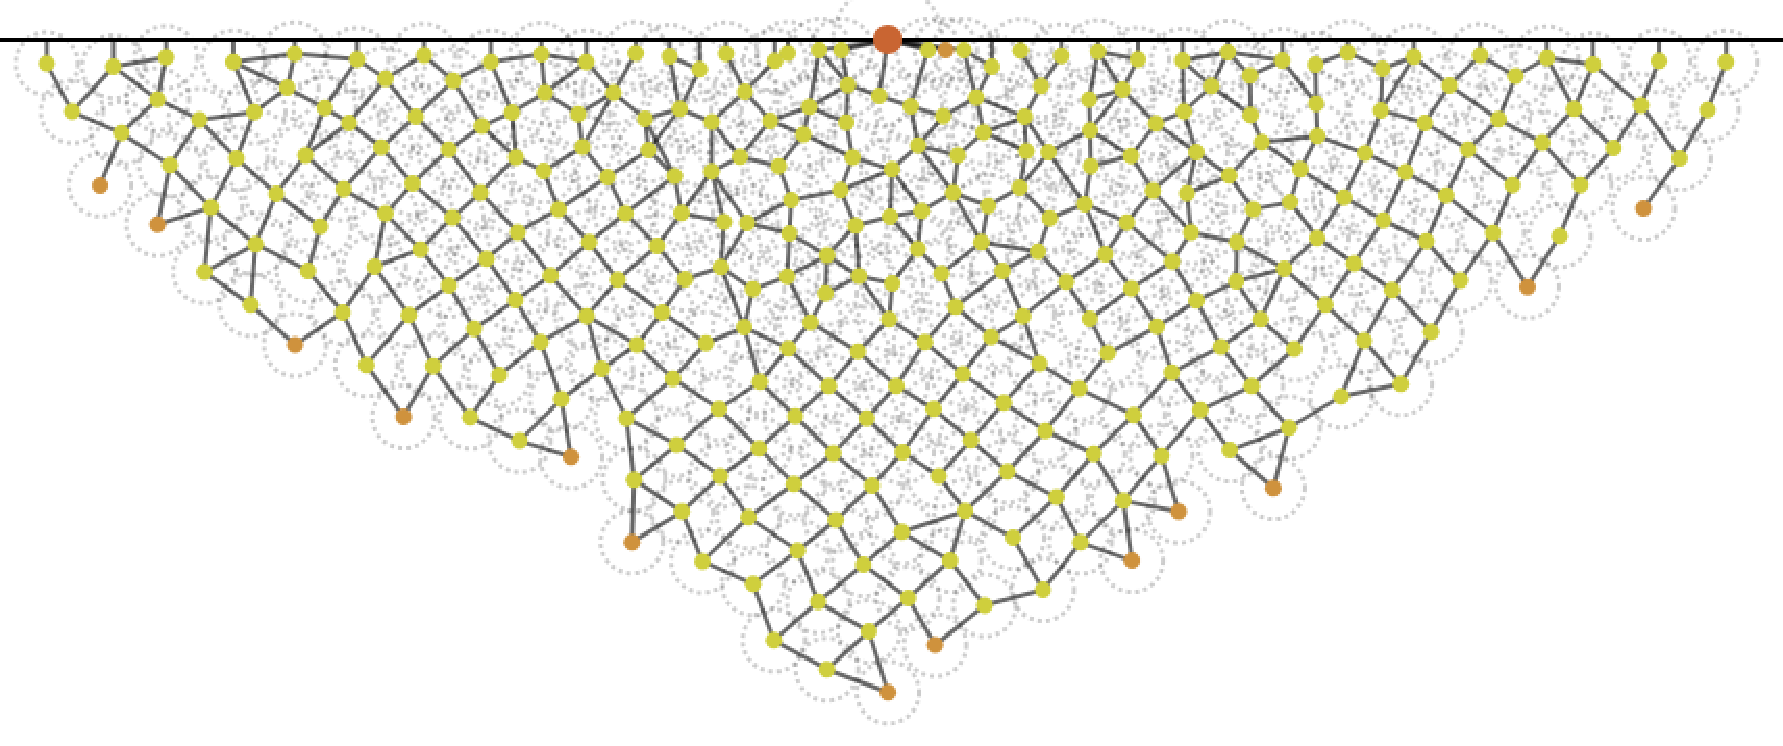
\includegraphics[width=\linewidth]{crawl_0.6_climb_0.6_size_0_mass_0_cnt_300.pdf}
        \caption{A $300$ bee structure ($\alpha = \beta = \sfrac{3}{5}$)}
        \label{fig:snapshot}
    \end{figure}

    More often than not, a stabilized structure looks like the one in \autoref{fig:snapshot}.
    To offer some context, the small inner circles have radius $r_{n}$ while the larger outer circles
    have radius $r_{b}$. The queen bee is the large glowing red circle at the core of the bivouac.
    Yellow bees are those that are supporting at least one bee, while red bees are those without
    any bees to support, and are therefore prime candidates to climb downwards as described earlier.

    One may observe that the outer regions are characterized by a diagonally-centered square
    lattice structure, whereas inner regions lack a discernible pattern. Additionally, outer
    regions are less dense compared to the tightly packed inner region. This is to be expected
    as you'd require more bees at the upper layers to support the weight of the layers below them.

    \subsection{Bee Count} \label{section:bee_count}

    To begin, we mirror the analysis in \cite{shishkov2022strength} by varying the bee count while
    keeping the other parameters constant ($\alpha = \beta = \sfrac{2}{5}$). In addition, we
    adopt the \textit{binning method} by collecting samples at distinct, uniform intervals down
    the vertical axis, which we'll denote as the depth $z$.

    \begin{figure}[H]
        \centering
        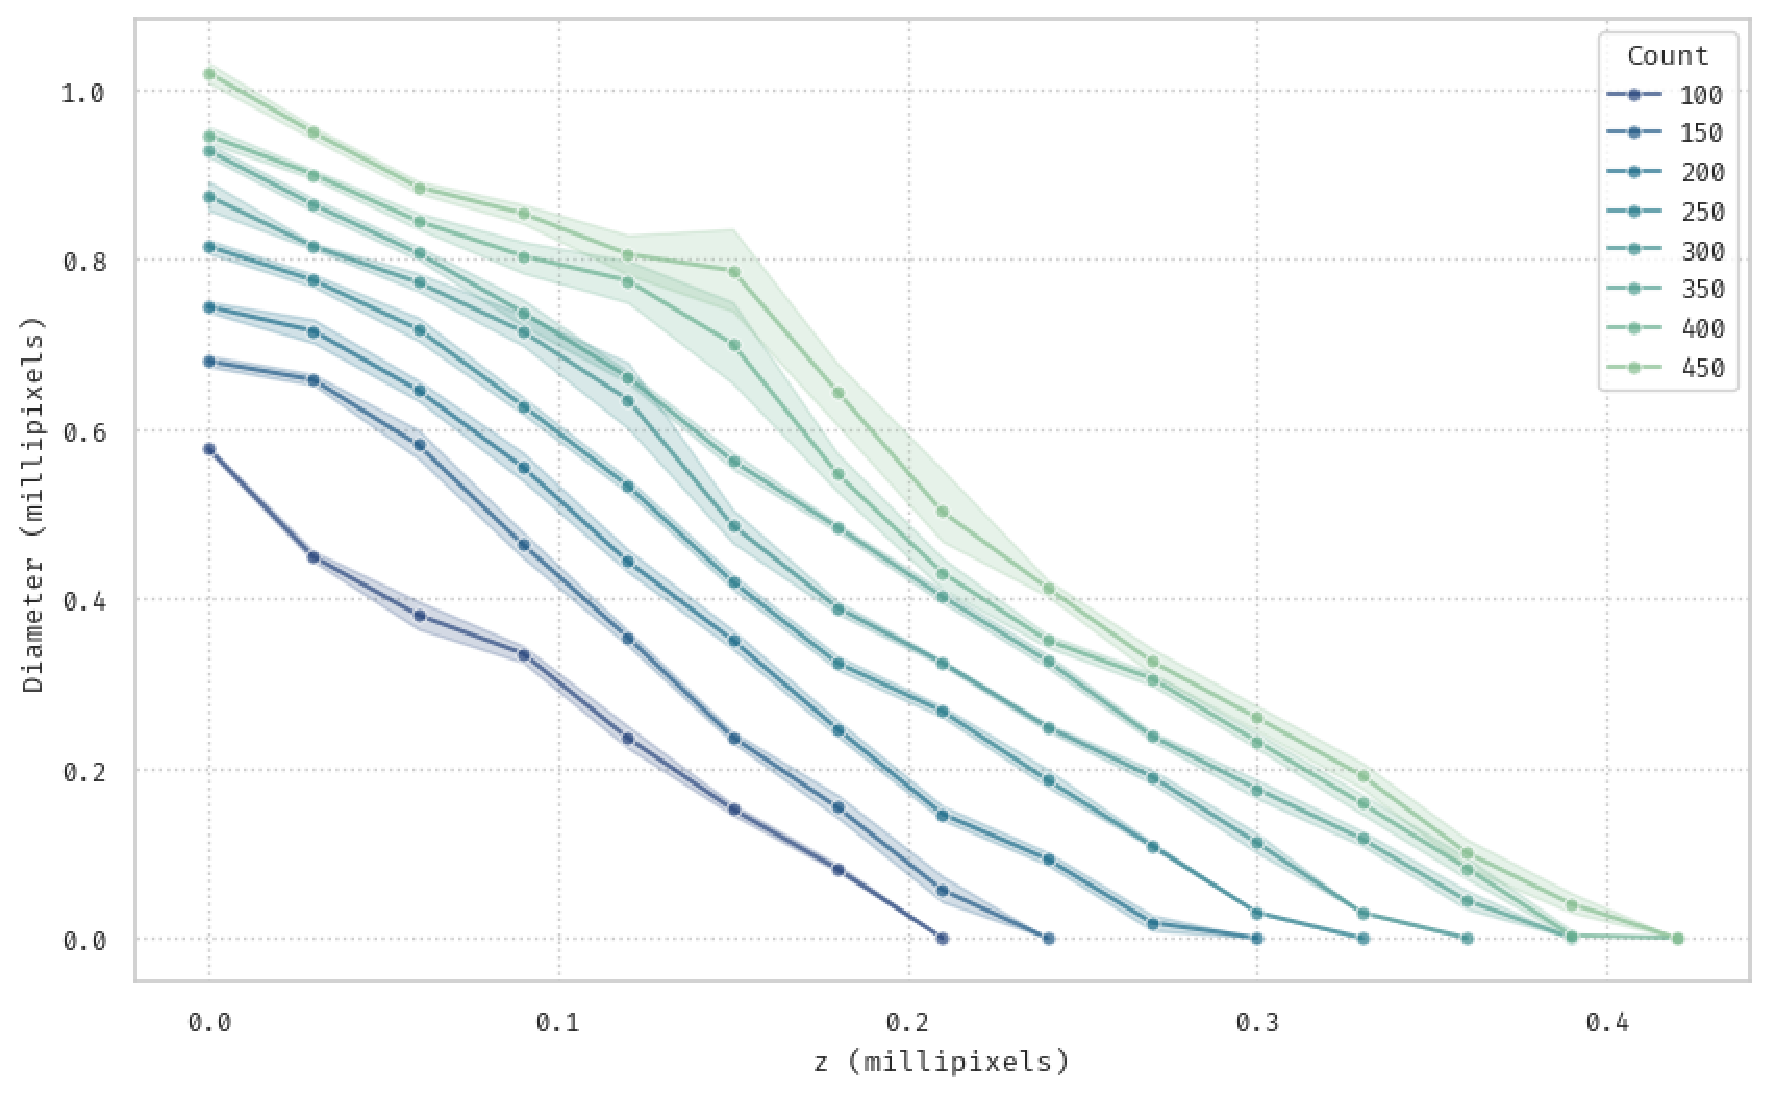
\includegraphics[width=\linewidth]{bee_count_diameter.pdf}
        \caption{Diameter against depth $z$}
        \label{fig:count_diameter_against_depth}
    \end{figure}

    From \autoref{fig:count_diameter_against_depth}, it appears that the diameter decreases almost
    linearly with depth $z$. However, this linear trend doesn't necessarily hold true for
    other parameter configurations as we'll discover subsequently.

    \begin{figure}[H]
        \centering
        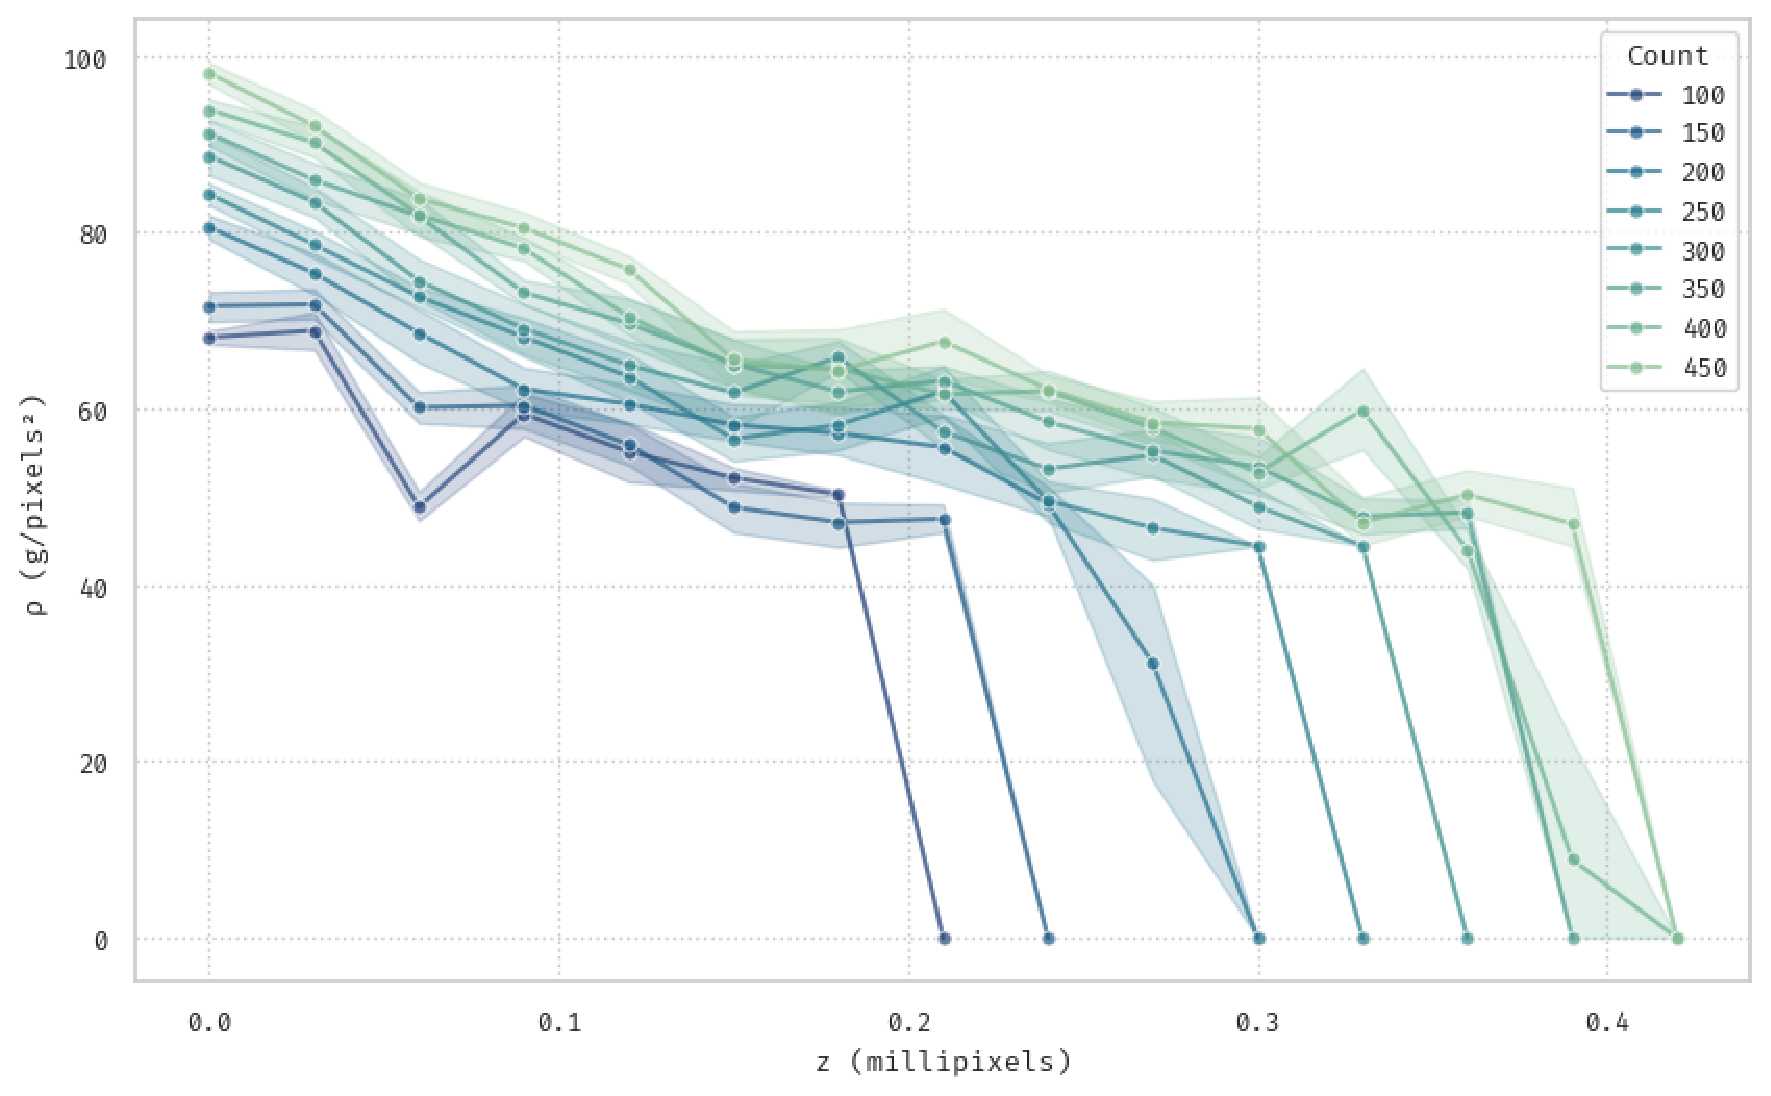
\includegraphics[width=\linewidth]{bee_count_density.pdf}
        \caption{Density $\rho$ against depth $z$}
        \label{fig:count_density_against_depth}
    \end{figure}

    Next, we examine how the density $p$ changes with $z$. From \autoref{fig:count_density_against_depth},
    a gentle linear downwards slope is prevalent at first. However, past a certain point, the density
    sharply dips to zero. As unintuitive as this appears, this result actually corroborate with
    those established in physical experiments \cite{shishkov2022strength}.

    \begin{figure}[H]
        \centering
        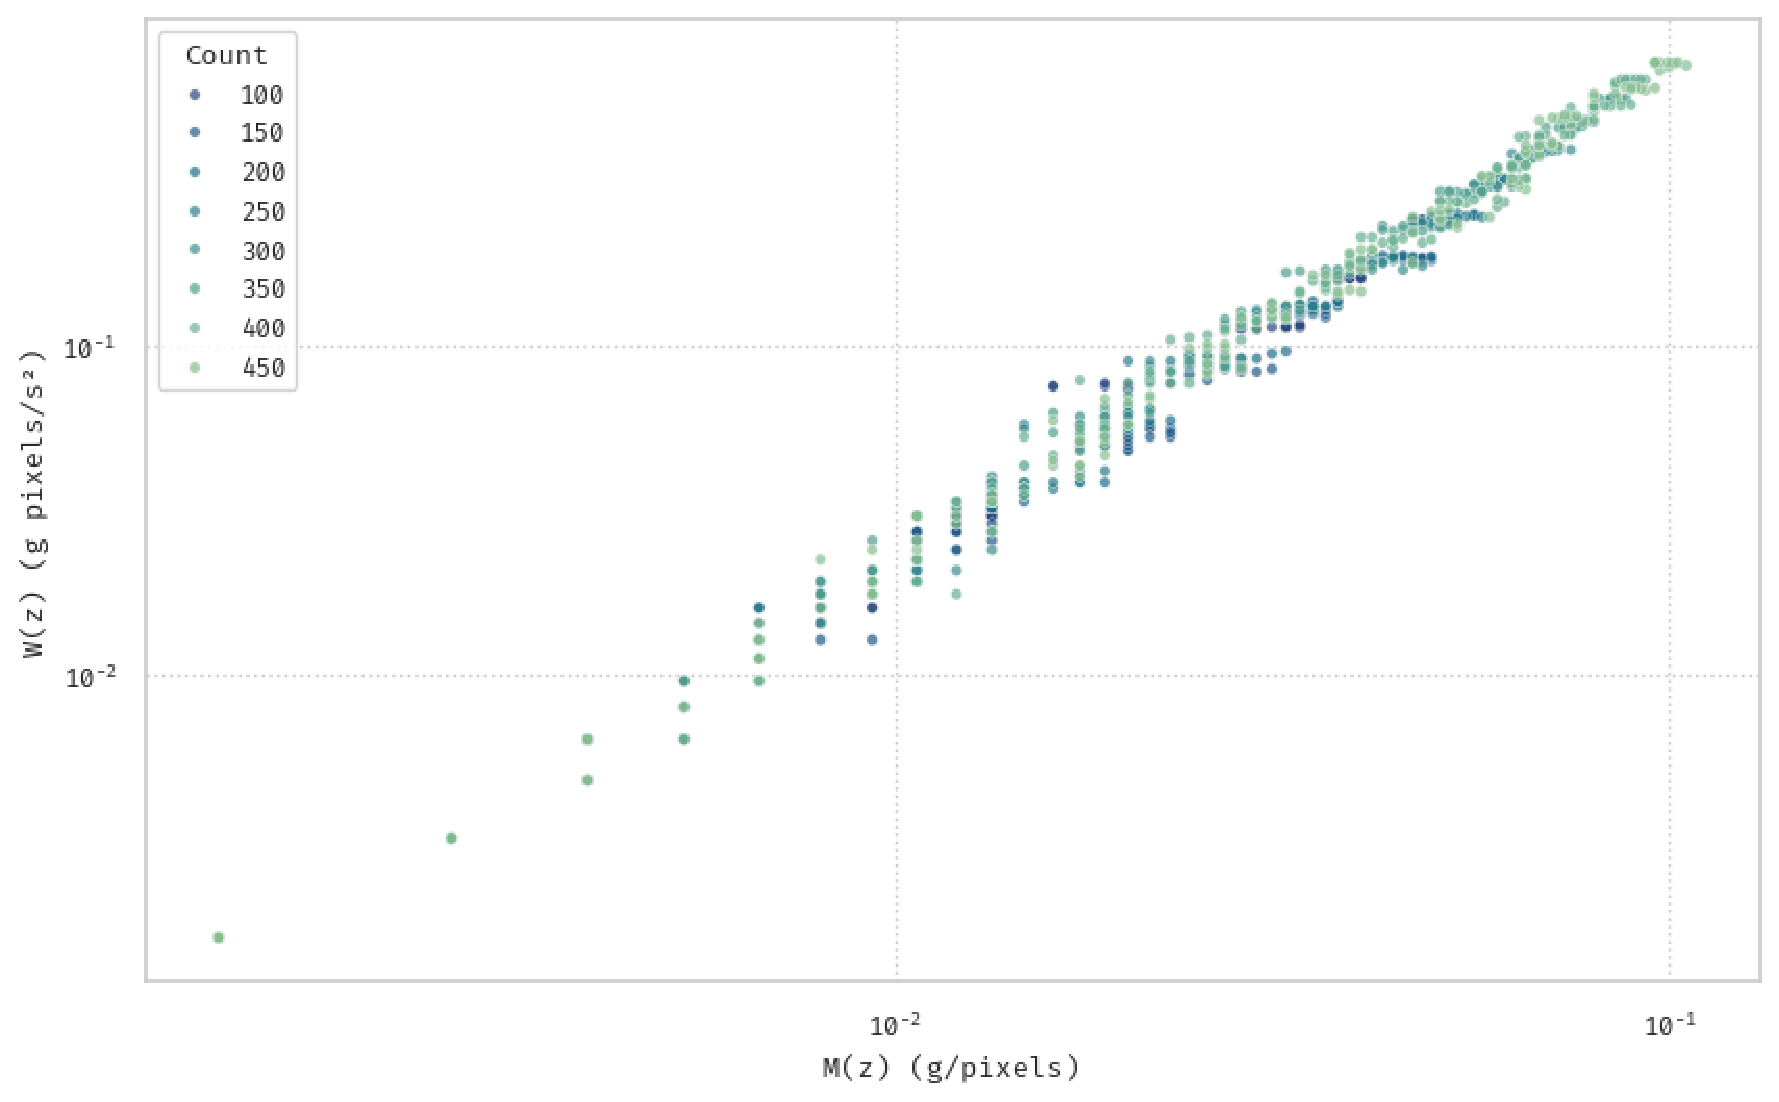
\includegraphics[width=\linewidth]{bee_count_weight.pdf}
        \caption{Supported weight $W$ against layer mass $M$}
        \label{fig:count_weight_against_mass}
    \end{figure}

    By defining the supported weight as the sum of the weight of the current layer along with all
    other layers below it, \autoref{fig:count_weight_against_mass} reveals that when a logarithmic scale is used,
    the supported weight appears to increase linearly with the mass of a layer. By fitting
    a power curve of the form $W = C \cdot M^{a}$, we are able to obtain \autoref{fig:count_power_law}.

    \begin{figure}[H]
        \centering
        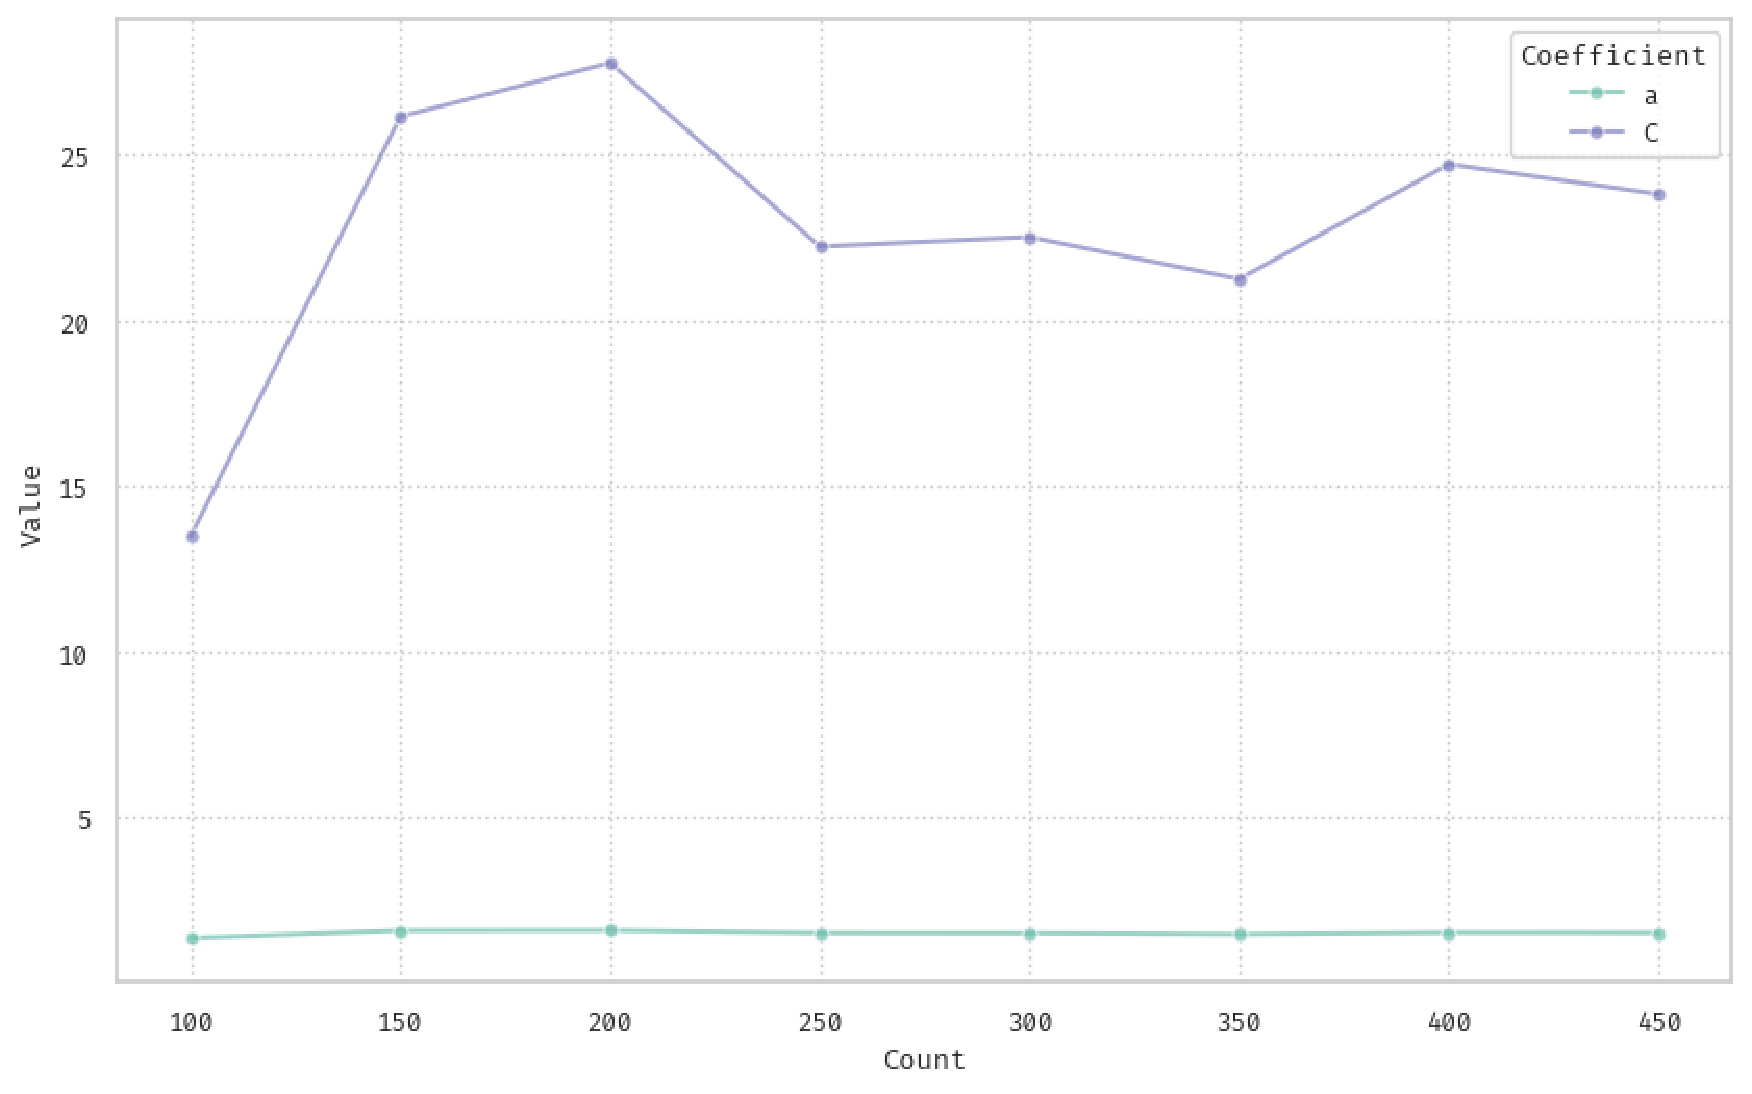
\includegraphics[width=\linewidth]{bee_count_power_law.pdf}
        \caption{Coefficients of Best Fit}
        \label{fig:count_power_law}
    \end{figure}

    Noting that $a$ is near-constant across different bee counts, we may deduce that our
    simulation does abide by the established strength-mass scaling law.

    \begin{figure}[H]
        \centering
        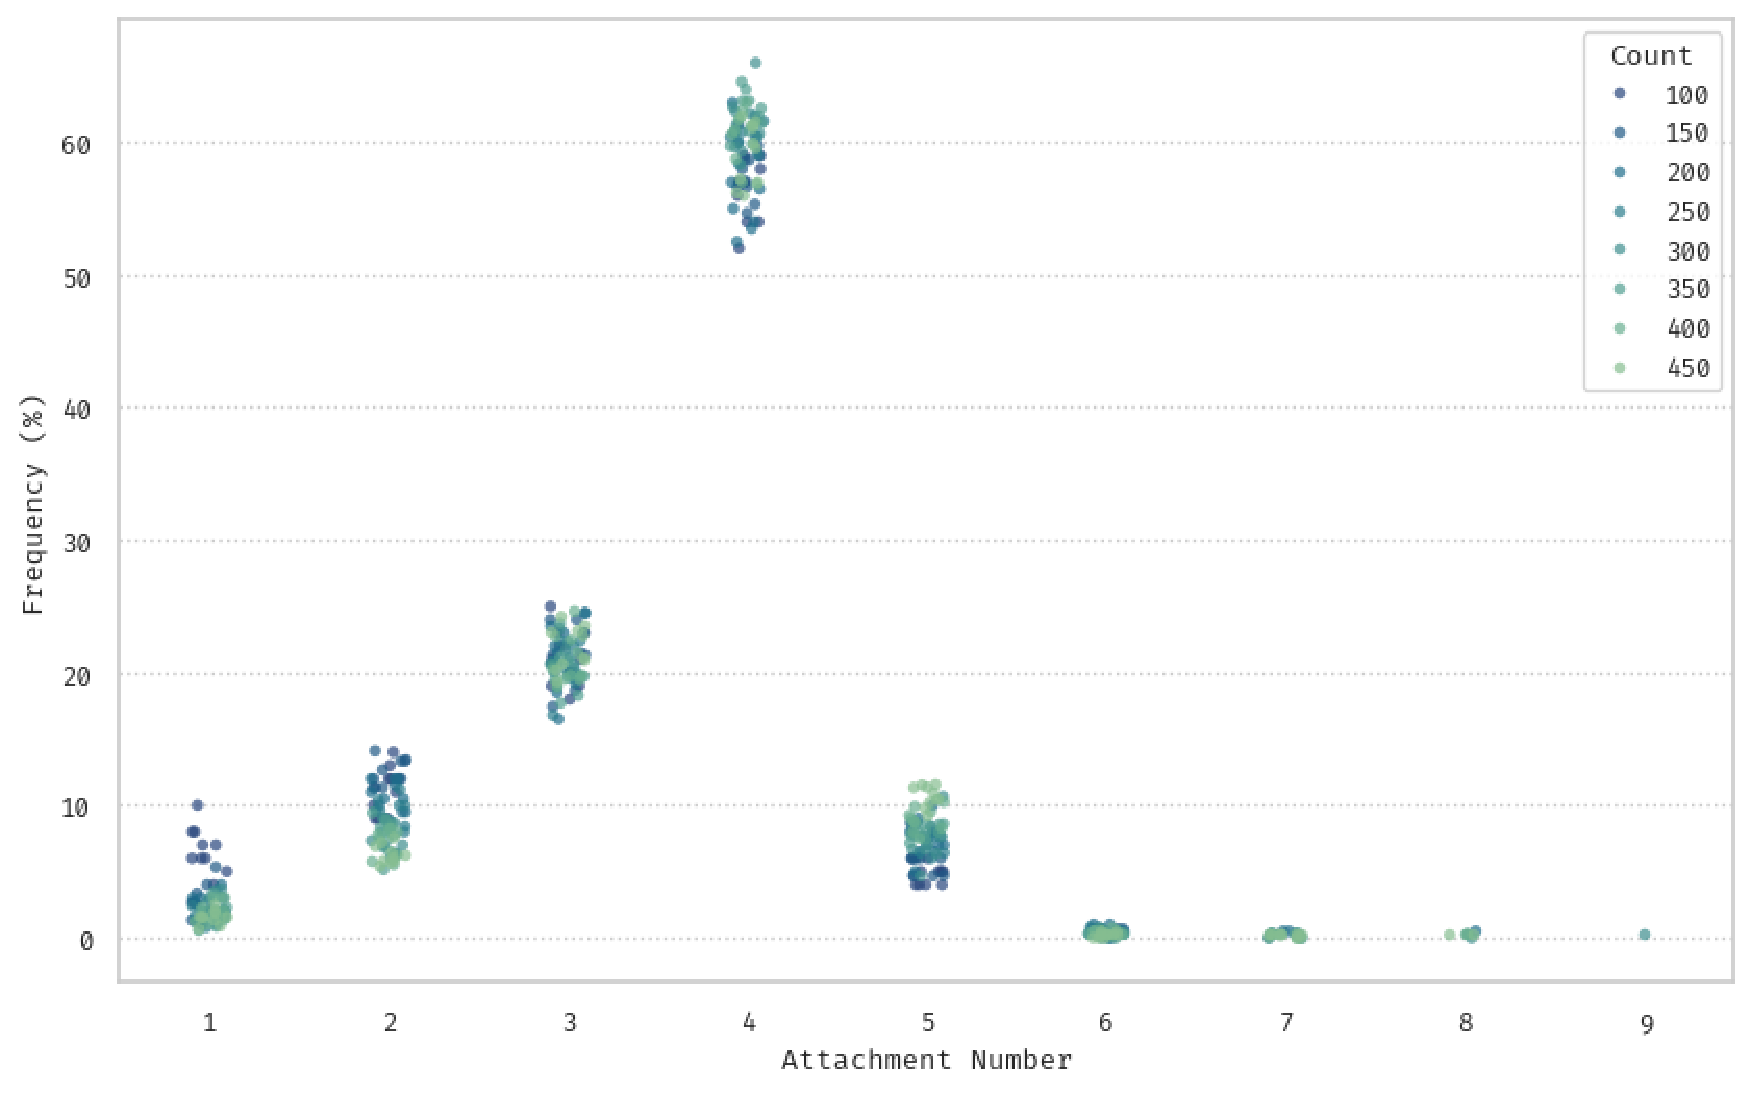
\includegraphics[width=\linewidth]{bee_count_distribution.pdf}
        \caption{Frequency against attach number}
        \label{fig:count_distribution}
    \end{figure}

    We have consolidated the frequency distribution across attachment numbers.
    We define the \textit{attachment number} as the sum of in-degrees and
    out-degrees, i.e., the total number of bees that a bee is attached to or is supporting.
    Referring to \autoref{fig:count_distribution}, it is evident that the predominant
    attachment number is \textit{four}, reflecting that the square lattice structure is
    the predominant structure.

    Another subtle observation is that as the number of
    bees increase, there's a slight shift towards higher attachment numbers, i.e., those
    above four. This may be explained by the need to have a large densely-packed base layer to
    support the heavier load.

    \subsection{Crawl Rate}

    In this section, we'll attempt to vary the crawl rate $\alpha$ while keeping the
    climb rate $\beta$ constant at $\sfrac{2}{5}$ and the number of bees constant at $250$.

    \begin{figure}[H]
        \centering
        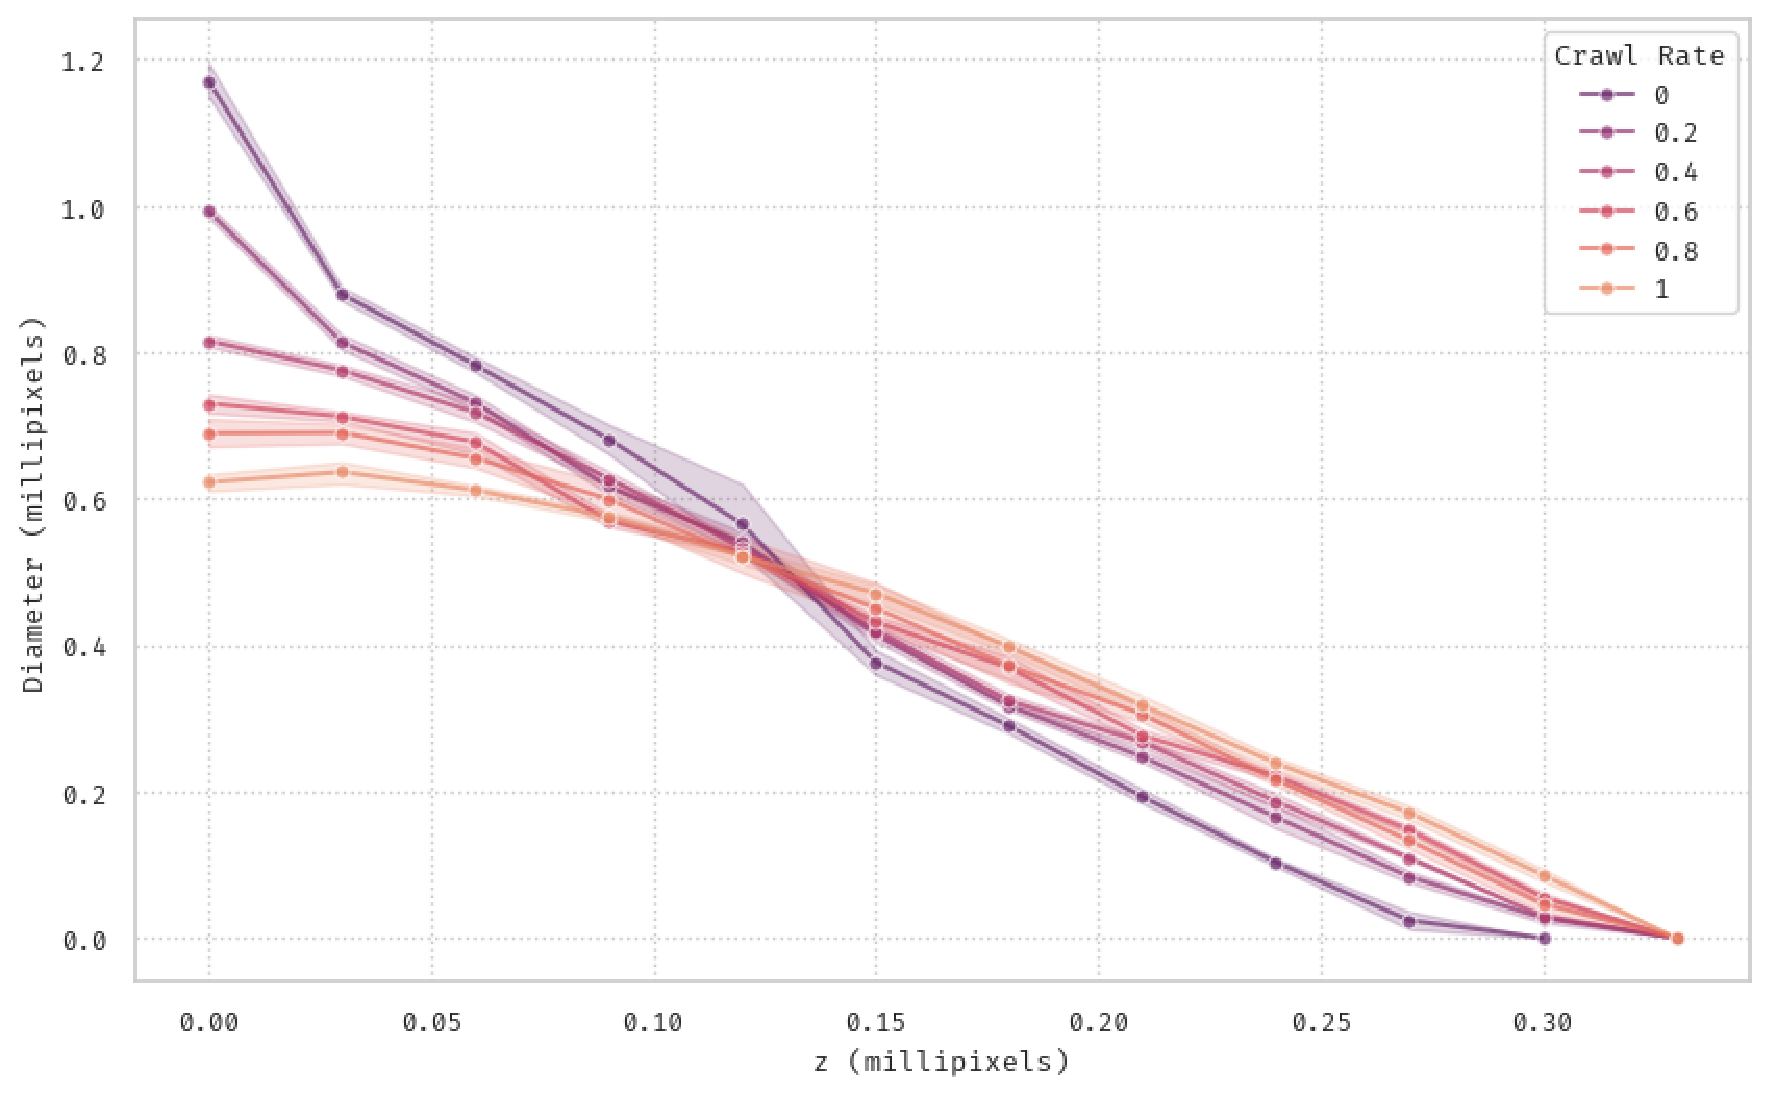
\includegraphics[width=\linewidth]{crawl_diameter.pdf}
        \caption{Diameter against depth $z$}
        \label{fig:crawl_diameter}
    \end{figure}

    \begin{figure}[H]
        \centering
        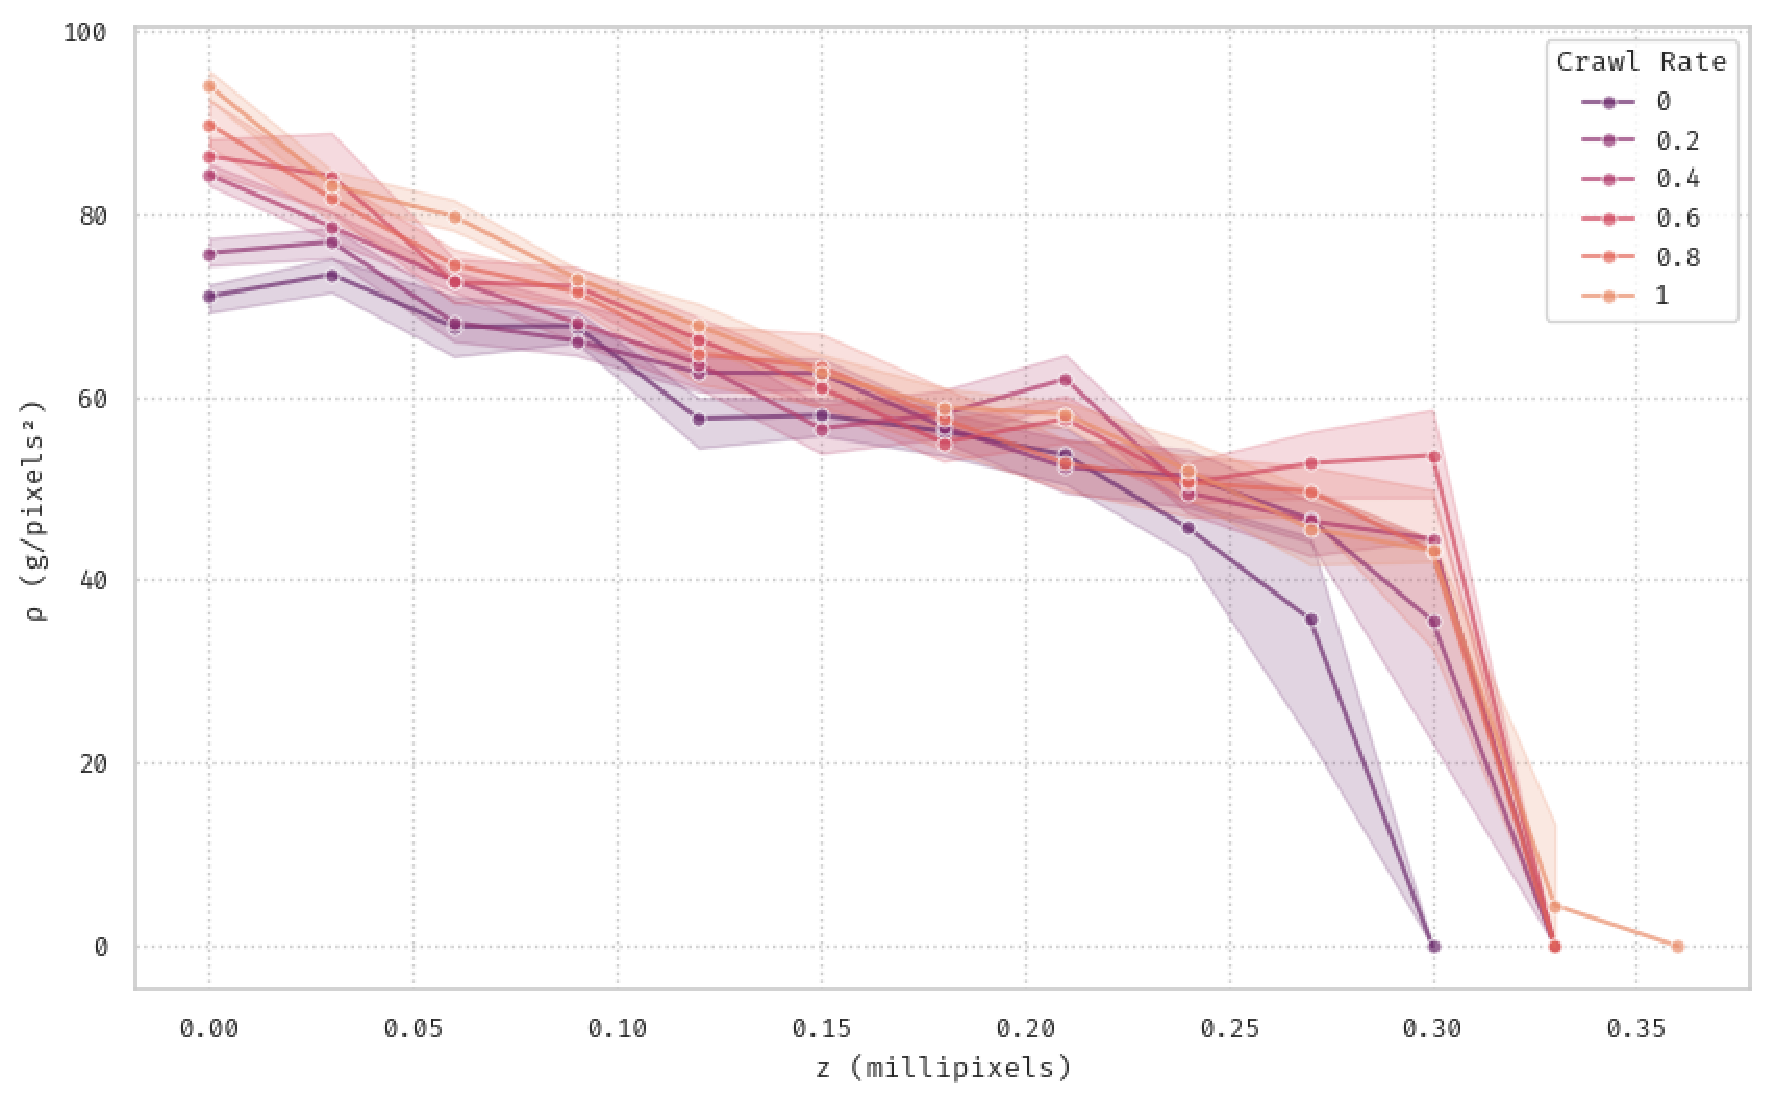
\includegraphics[width=\linewidth]{crawl_density.pdf}
        \caption{Density $\rho$ against depth $z$}
        \label{fig:crawl_density}
    \end{figure}

    At first glance, \autoref{fig:crawl_diameter} and \autoref{fig:crawl_density} both
    present a similar overall structure that we've come to know from \autoref{section:bee_count}.
    However, it's worth noting how muted the impact of $\alpha$ is at influencing both the overall
    shape and density of the bivouac. Even, as we tune $\alpha$ from zero all the way to one,
    it appears that the bees only react slightly.

    This isn't surprising considering $\alpha$
    only affects those attached to the board, which is just a fraction of the overall swarm,
    so much of the impact would be concentrated at the base layer. By focusing on low values of $z$ in
    \autoref{fig:crawl_diameter}, it's clear that $\alpha$ plays an important role at the
    bottom layers.

    \subsection{Climb Rate}

    \begin{figure}[H]
        \centering
        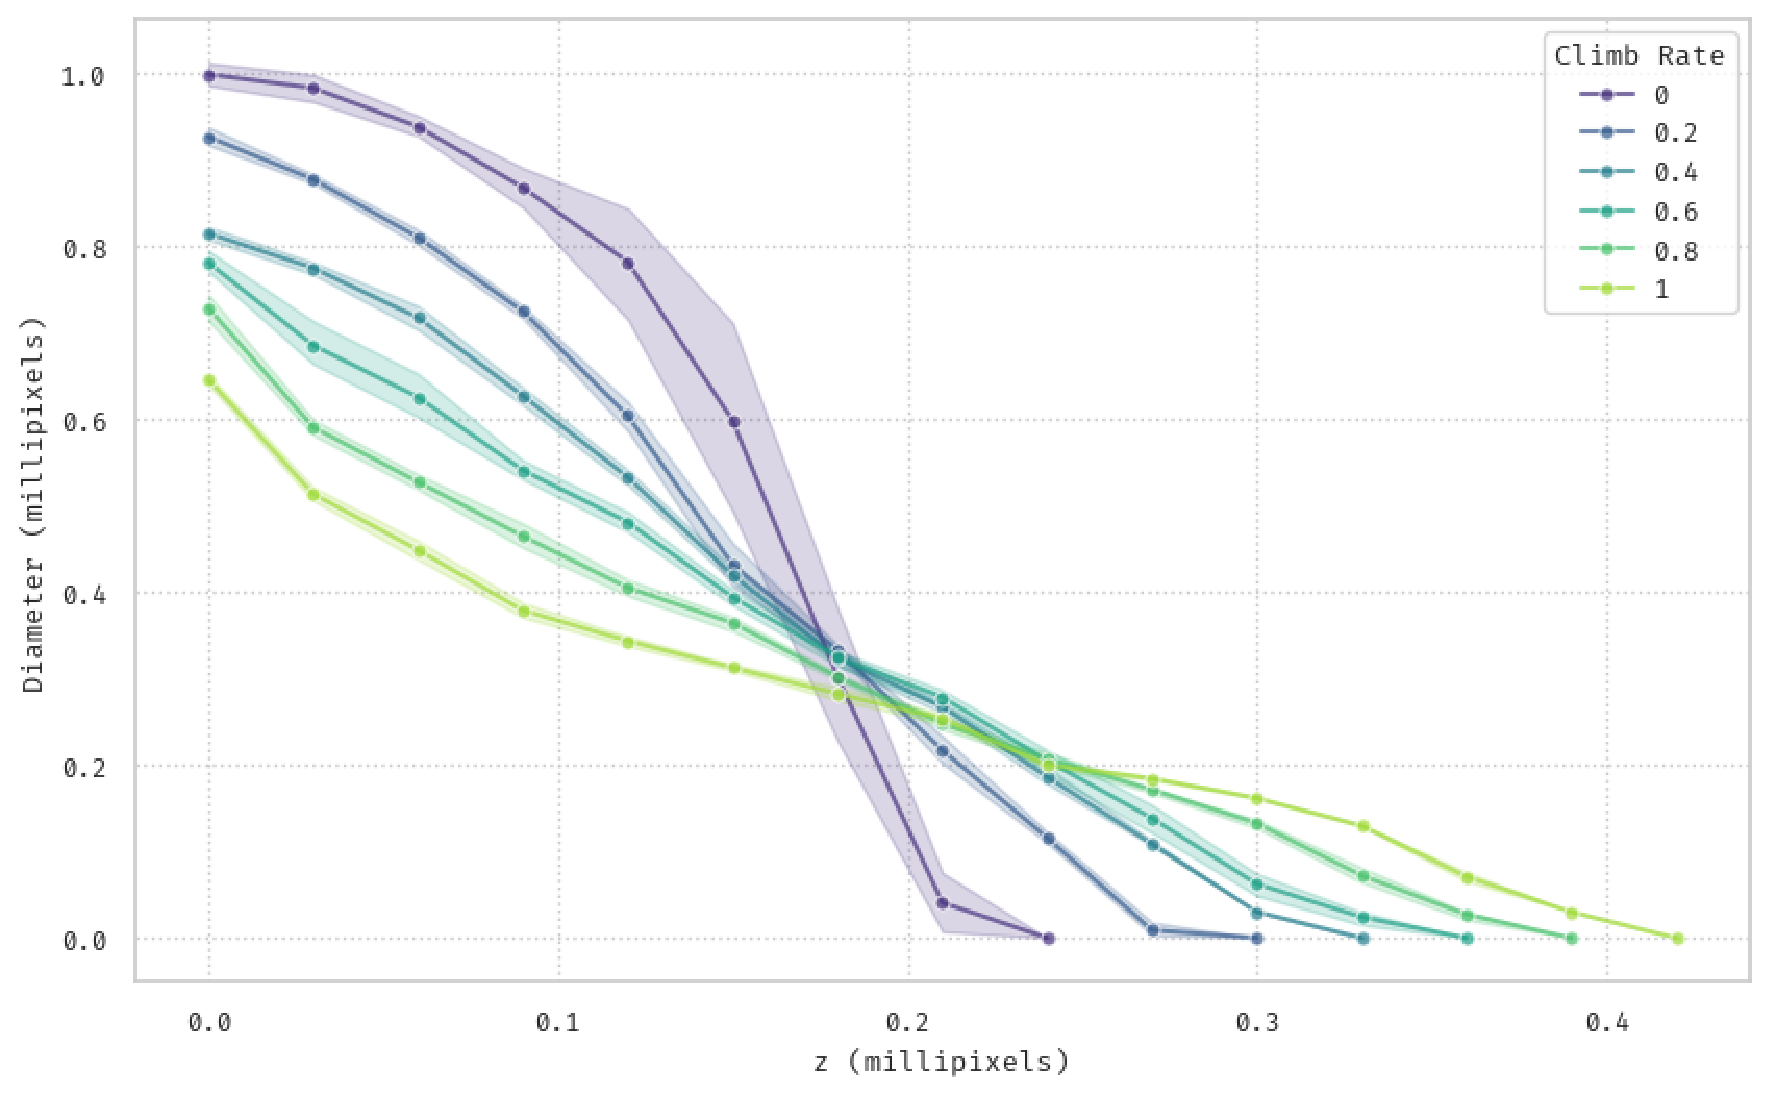
\includegraphics[width=\linewidth]{climb_diameter.pdf}
        \caption{Diameter against depth $z$}
        \label{fig:climb_diameter}
    \end{figure}

    Through \autoref{fig:climb_diameter} and \autoref{fig:climb_density}, we reveal a
    stark difference between the crawl and climb rates, in the sense that small
    perturbations in $\beta$ have a massive impact on the morphology of the structure.
    Intuitively, as the bees try to climb the mount more vigorously, it's only
    logical for a pointy densely-packed formation to be the result.


    \begin{figure}[H]
        \centering
        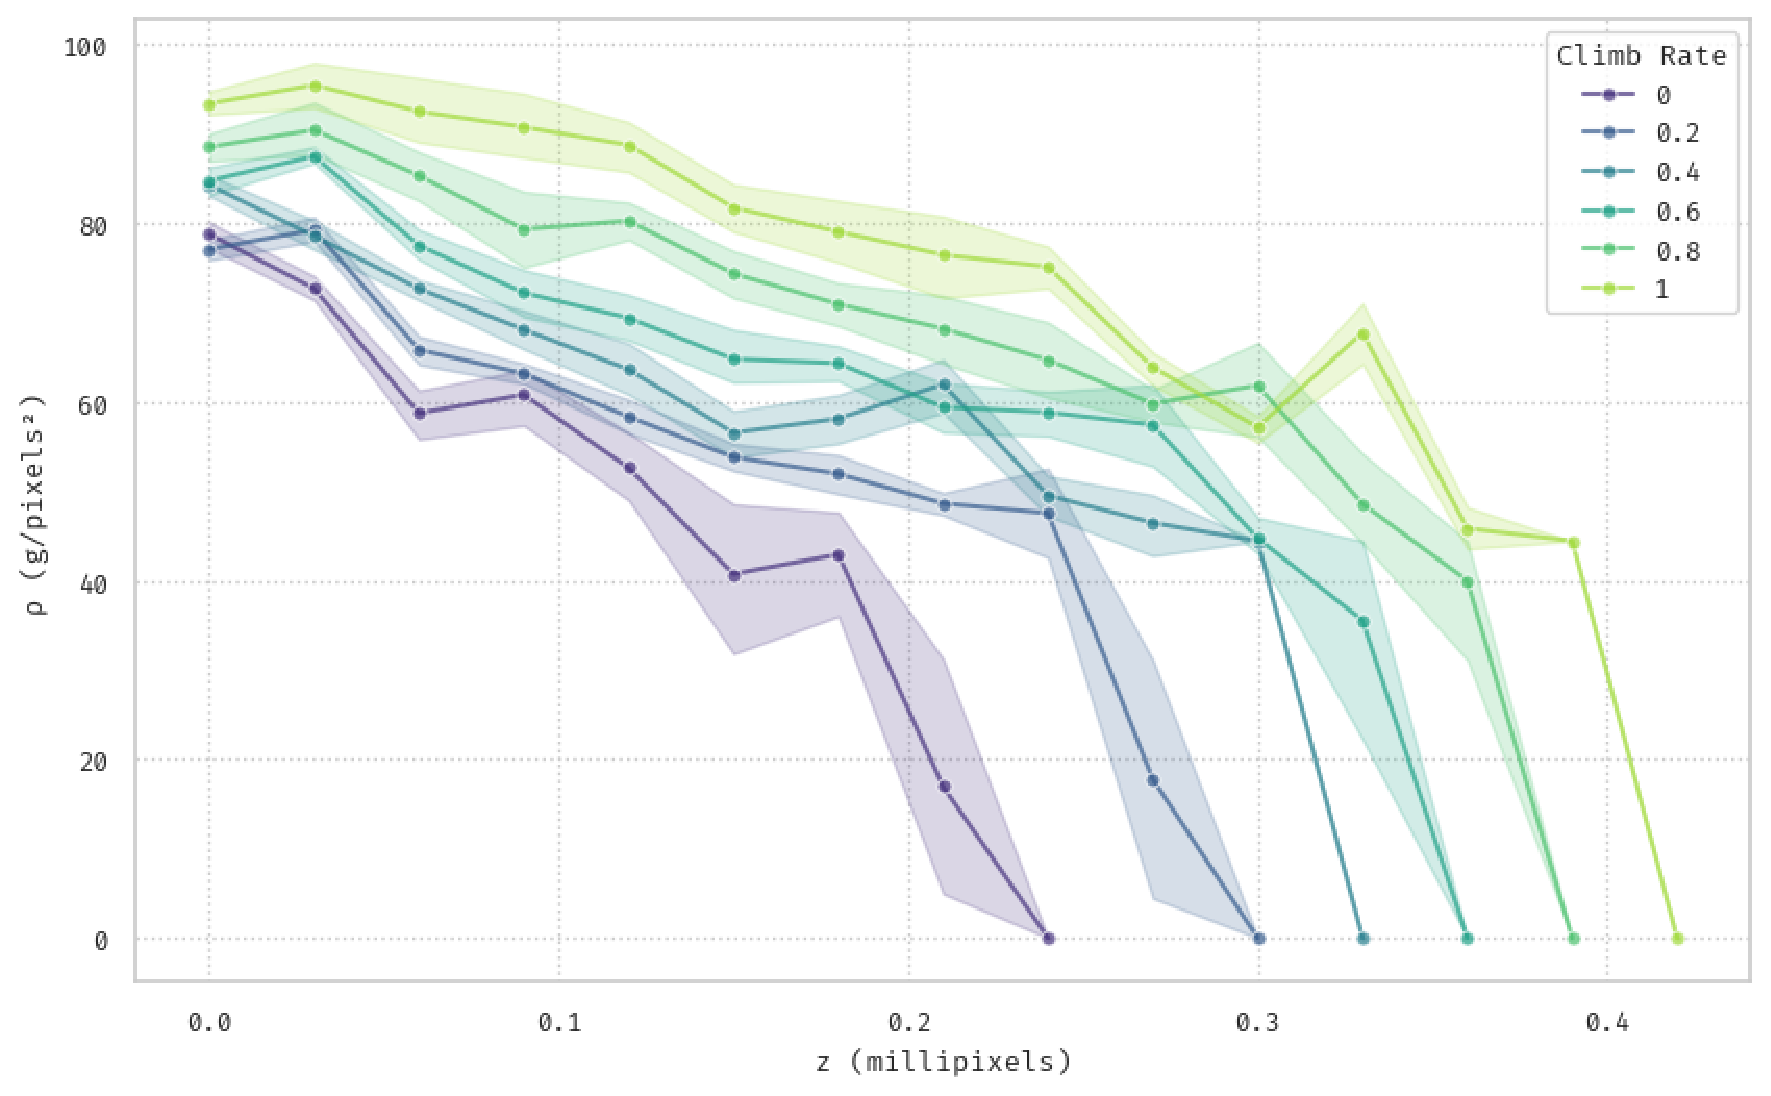
\includegraphics[width=\linewidth]{climb_density.pdf}
        \caption{Density $\rho$ against depth $z$}
        \label{fig:climb_density}
    \end{figure}

    \subsection{Phase Diagram}

    Thus far, we've only considered $\alpha$ and $\beta$ independently. However, that does not
    paint a complete picture of the full range of morphologies that our simulation
    is able to produce. As such, let's vary both $\alpha$ and $\beta$ at the same
    time and observe the resulting bivouac structures. Additionally, we'll be keeping
    the number of bees constant at $100$.

    \begin{figure}[H]
        \centering
        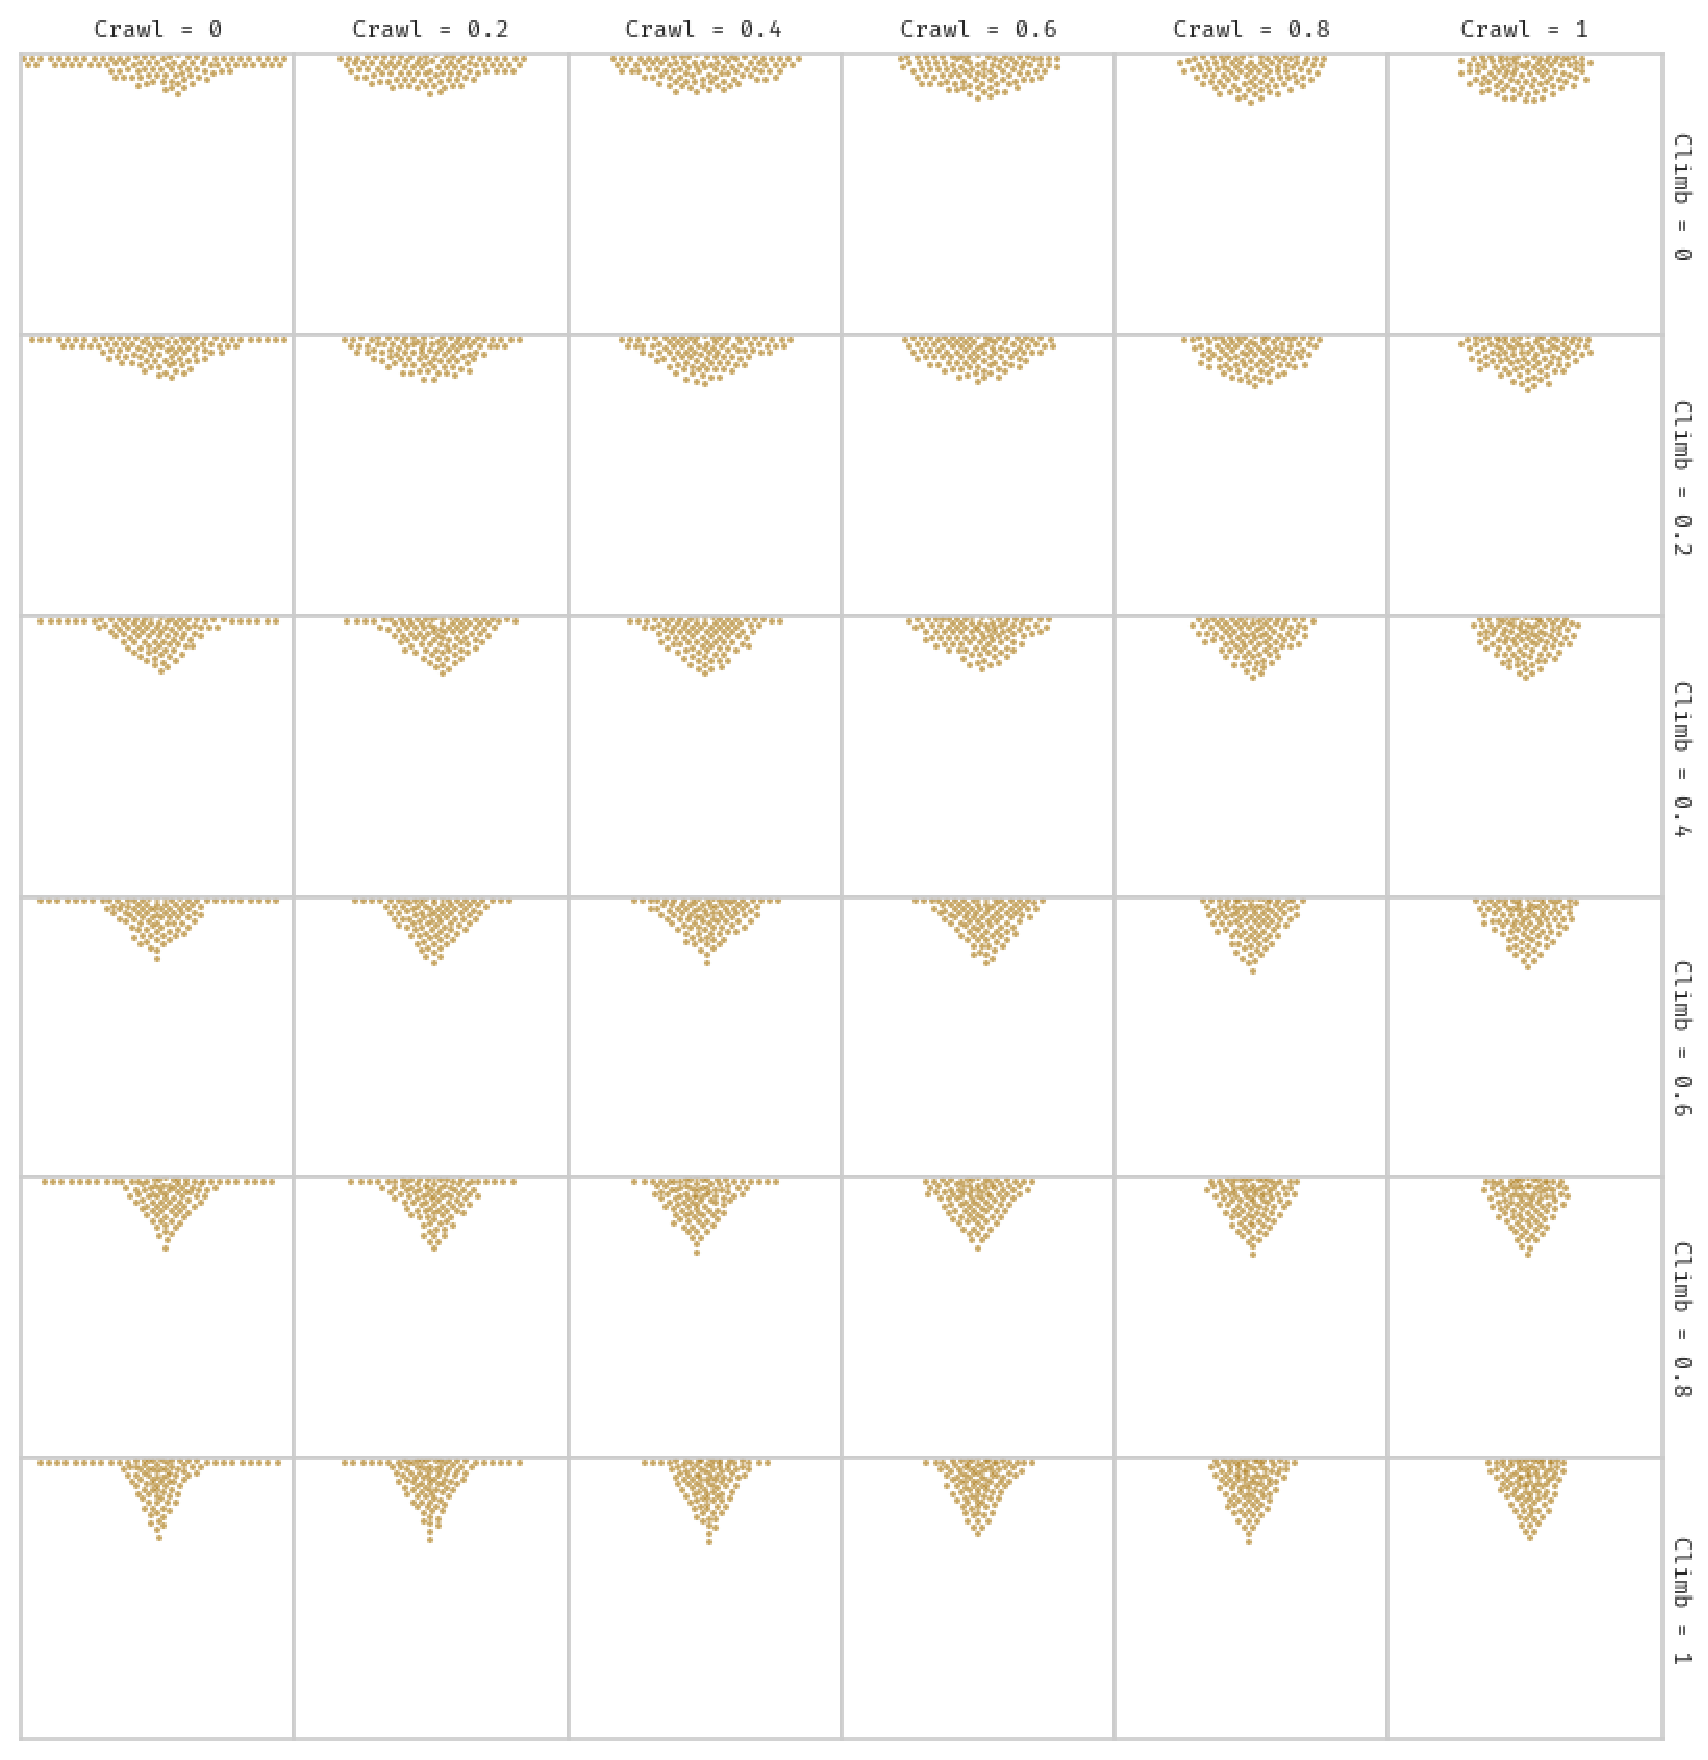
\includegraphics[width=\linewidth]{phase_diagram.pdf}
        \caption{Phase Diagram}
        \label{fig:phase_diagram}
    \end{figure}

    With reference to \autoref{fig:phase_diagram}, we may now inspect the entire spectrum of
    states. As alluded to earlier, it holds that $\beta$ is the dominant parameter in the
    simulation. Another observation is that an ideal parameter configuration would be
    around $\alpha = \beta = \sfrac{2}{5}$, as that morphology resembles what we observe in
    physical experiments conducted in \cite{peleg2018collective}.

    Another remarkable property is that the real-life parameter \textit{temperature}
    may in fact be a linear combination of $\alpha$ and $\beta$. According to physical experiments,
    swarm morphologies exist as means for temperature regulation \cite{heinrich1981mechanisms}.
    Low temperatures produce structures with a higher $\alpha$ and a low $\beta$, whereas
    high temperatures work in reverse, producing more pointy structures with a low $\alpha$
    and a high $\beta$.

    \begin{figure}[H]
        \centering
        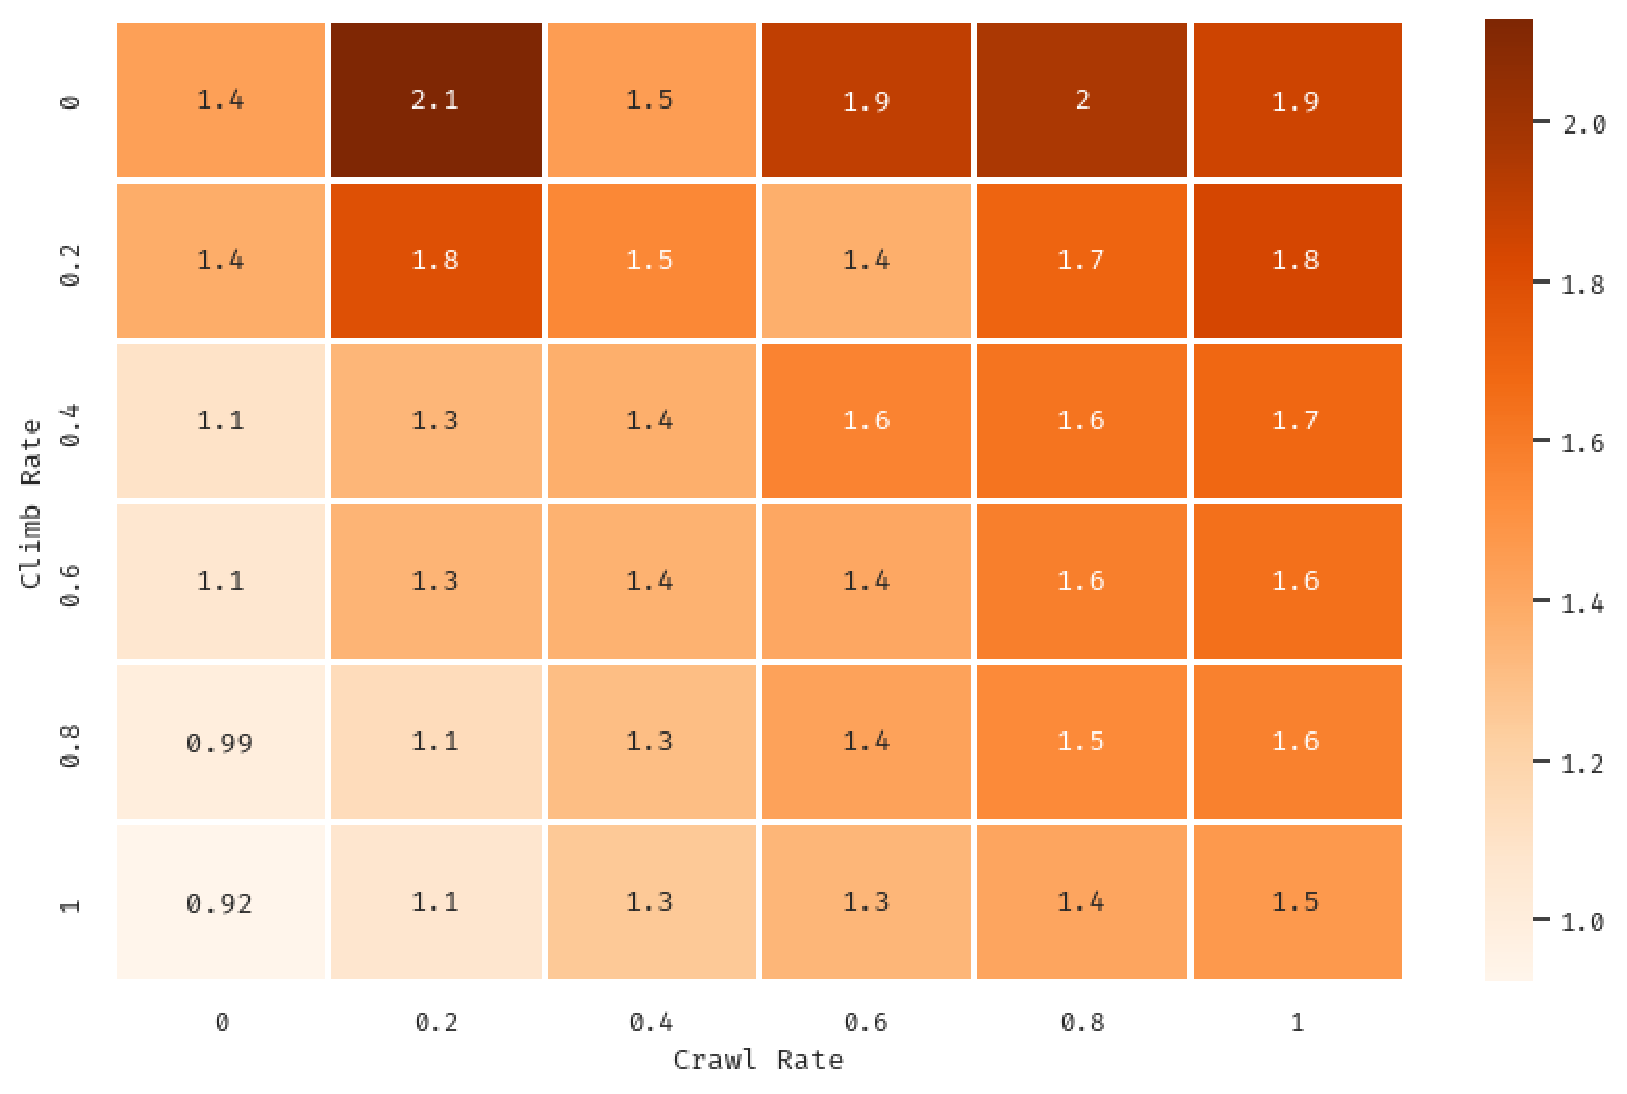
\includegraphics[width=\linewidth]{heatmap.pdf}
        \caption{Heatmap of $a$ coefficients}
        \label{fig:heatmap}
    \end{figure}

    Besides looking at the shape of the bivouacs, we may also examine how the $a$
    coefficient changes when we fit the power curve. In \autoref{fig:heatmap}, it's evident
    that higher crawl rate configurations result in larger $a$, suggesting that each layer
    is supporting far more weight in these pointy structures.

    \section{Conclusion}

    From our analysis, it appears that the simple rules we've designed were able to yield
    results that corroborate with real-life findings. Additionally, the simulation may be
    extended upon to explore how other parameters such as the \textit{curvature} is
    changing over time.

    There are several limitations to this study. Firstly, the nature of this research is
    very experimental, i.e., a lot of trial and error is required to find the right parameter
    values and the right formulas, and the ones that we've suggested may not be the only ones that
    could potentially work. The state space of possible combinations is simply too large to cover,
    so it's likely that we've inevitably missed more optimal configurations. Secondly, we lack
    comprehensive information on the \textit{internal} structure of the bivouac, hence we can't verify
    the accuracy of the diagonally-centered square lattice structure that our model yields.

    Moving forward, we hope to work on a three-dimensional variation of this model. We believe this
    is possible through better optimization techniques, and more importantly, with the assistance
    of Dr. Orit Peleg from the University of Colorado Boulder, we are able to receive more information
    on the structure of the bivouacs in the future. With the development of a three-dimensional model,
    we can then better compare our findings (such as the $\alpha$ coefficient) with the established values
    in the literature.

    \section*{Acknowledgments}

    I would like to acknowledge the funding support from Nanyang Technological University – URECA Undergraduate Research Programme for this research project.

    In addition, I would also like to thank Ph.D student Donn Liew for offering advice and giving me an initial
    version of the 2D simulation (written in Python), which I used as inspiration throughout the URECA project.

    Next, I would like to thank Prof Yong (my mentor) for his extensive guidance throughout the past year. His
    teachings and feedback have allowed the model to become what it is today.

    Finally, I want to thank Dr. Orit Peleg for providing the key video recording upon which we've modeled the simulation after.

    \section*{Appendix}

    So far, we've assumed that the worker bees are homogeneous in terms of both size and mass. However,
    in nature, it's likely for small variations to exist within the worker bees. For simplicity, let's try
    to use the Box-Muller transformation to retrieve a random value $b$ from zero to one \cite{box1958note}.
    Now, suppose we want to generate a value $r$ in the range $[1-\delta, 1+\delta]$, where $\delta \in (0, 1)$, we may retrive
    it using $r = 2b\delta + (1 - \delta)$. This $r$ may then be multiplied with the base values
    of either mass or ratio that we've established earlier, producing a range of different kinds of bees.

    \begin{figure}[H]
        \centering
        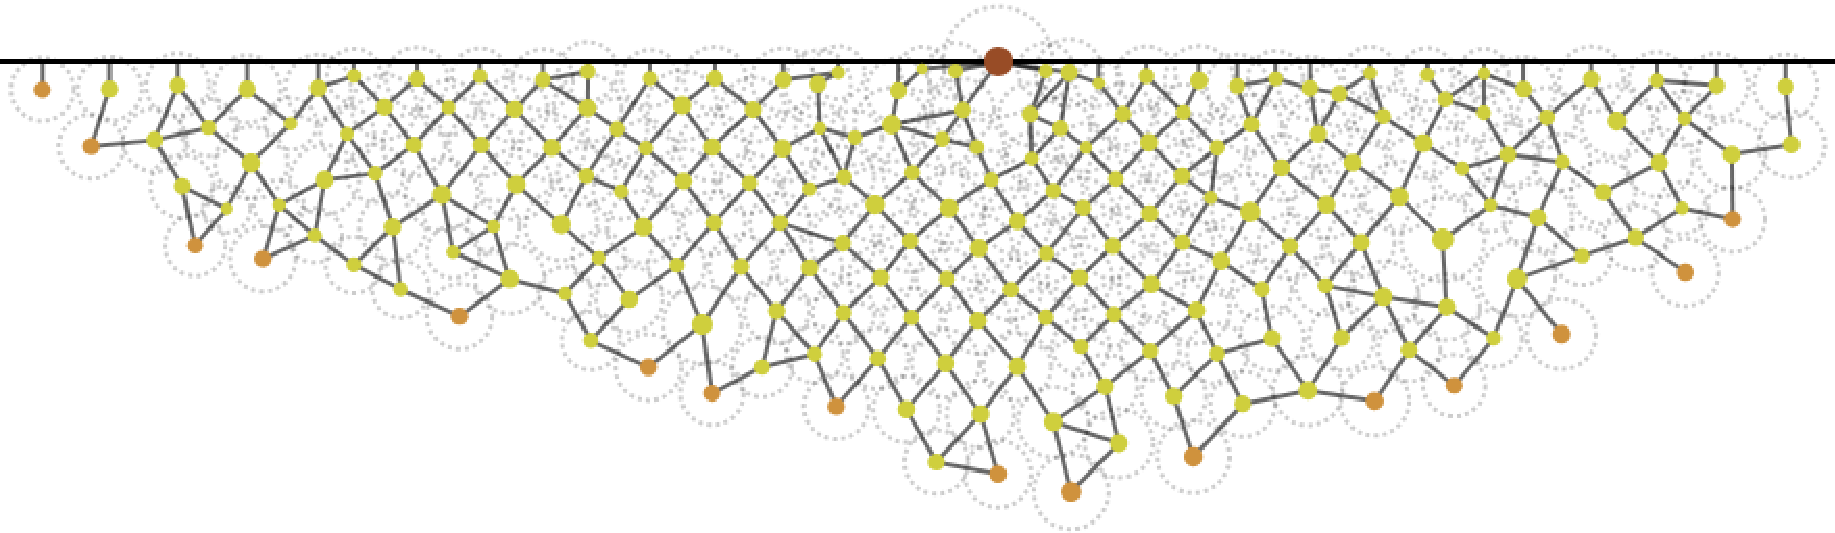
\includegraphics[width=\linewidth]{size_delta.pdf}
        \caption{A bivouac with a size delta of $\sfrac{1}{2}$}
        \label{fig:size_delta}
    \end{figure}

    From \autoref{fig:size_delta}, one may observe that the larger bees seem to be more prevalent around
    the perimeter of the bivouac. That's not to discount the fact that there are several large bees nested
    within the structure; but intuitively, it makes sense to have smaller bees near the core to provide
    a denser layer that's capable of supporting more bees. Note that a larger bee does not necessary
    mean a stronger one, it only implies that it takes up more space.

    \begin{figure}[H]
        \centering
        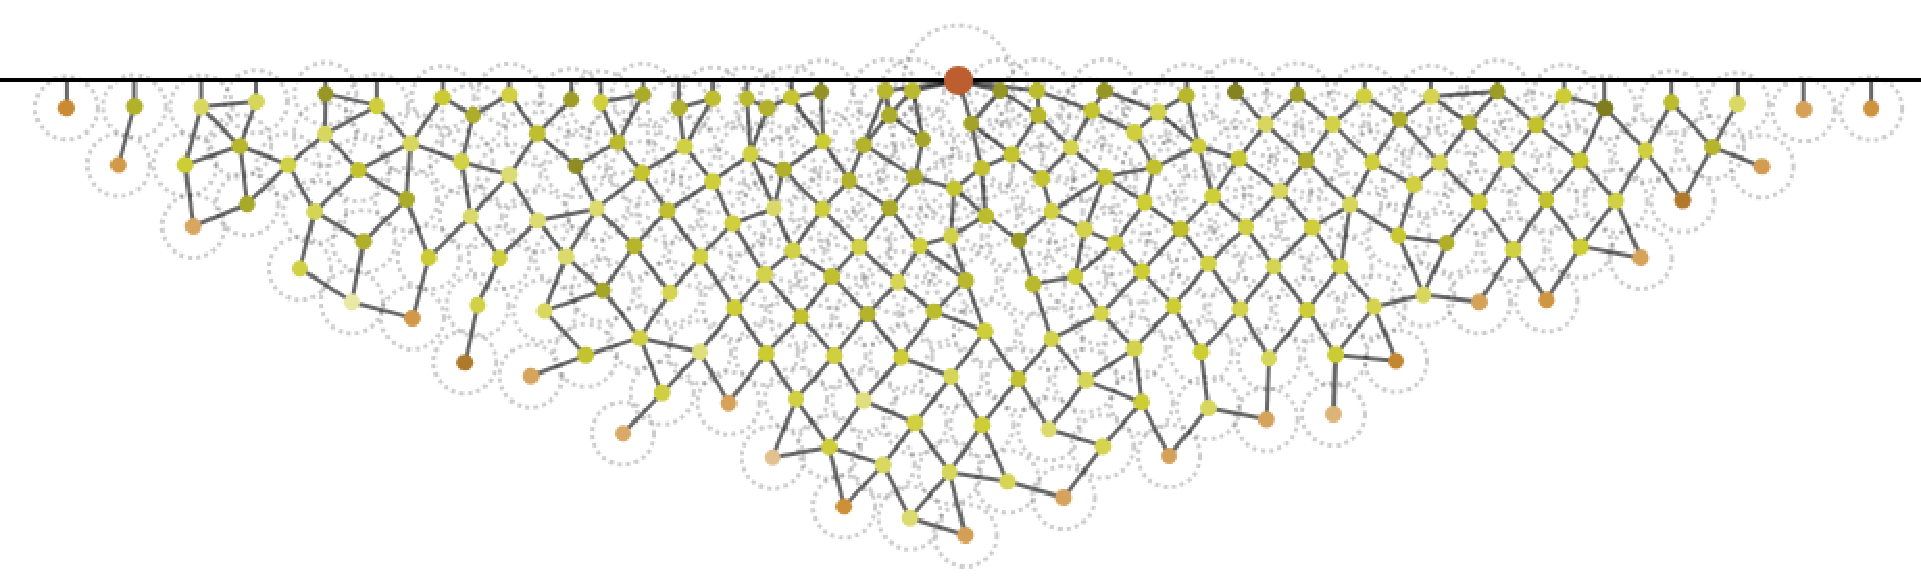
\includegraphics[width=\linewidth]{mass_delta.pdf}
        \caption{A bivouac with a mass delta of $\sfrac{1}{2}$}
        \label{fig:mass_delta}
    \end{figure}

    \autoref{fig:mass_delta} reveals that the heavier bees (indicated by the darker shade) tend to be situated
    near the queen. This is natural because even in the simplest case of a chain consisting of two bees, it would
    make sense for the heavier bee to be supporting the lighter one, not the other way around. Therefore, having
    the heavy bees clustered in the upper layers creates a more preferrable stable structure.

    \bibliographystyle{plain}  % Use an appropriate style (plainnat, abbrvnat, etc.)
    \bibliography{references}  % This refers to references.bib (without .bib extension)

\end{multicols}
\end{document}
